% Options for packages loaded elsewhere
\PassOptionsToPackage{unicode}{hyperref}
\PassOptionsToPackage{hyphens}{url}
\PassOptionsToPackage{dvipsnames,svgnames,x11names}{xcolor}
%
\documentclass[
  letterpaper,
  DIV=11,
  numbers=noendperiod,
  oneside]{scrartcl}

\usepackage{amsmath,amssymb}
\usepackage{iftex}
\ifPDFTeX
  \usepackage[T1]{fontenc}
  \usepackage[utf8]{inputenc}
  \usepackage{textcomp} % provide euro and other symbols
\else % if luatex or xetex
  \usepackage{unicode-math}
  \defaultfontfeatures{Scale=MatchLowercase}
  \defaultfontfeatures[\rmfamily]{Ligatures=TeX,Scale=1}
\fi
\usepackage{lmodern}
\ifPDFTeX\else  
    % xetex/luatex font selection
\fi
% Use upquote if available, for straight quotes in verbatim environments
\IfFileExists{upquote.sty}{\usepackage{upquote}}{}
\IfFileExists{microtype.sty}{% use microtype if available
  \usepackage[]{microtype}
  \UseMicrotypeSet[protrusion]{basicmath} % disable protrusion for tt fonts
}{}
\makeatletter
\@ifundefined{KOMAClassName}{% if non-KOMA class
  \IfFileExists{parskip.sty}{%
    \usepackage{parskip}
  }{% else
    \setlength{\parindent}{0pt}
    \setlength{\parskip}{6pt plus 2pt minus 1pt}}
}{% if KOMA class
  \KOMAoptions{parskip=half}}
\makeatother
\usepackage{xcolor}
\usepackage[left=1in,marginparwidth=2.0666666666667in,textwidth=4.1333333333333in,marginparsep=0.3in]{geometry}
\setlength{\emergencystretch}{3em} % prevent overfull lines
\setcounter{secnumdepth}{-\maxdimen} % remove section numbering
% Make \paragraph and \subparagraph free-standing
\ifx\paragraph\undefined\else
  \let\oldparagraph\paragraph
  \renewcommand{\paragraph}[1]{\oldparagraph{#1}\mbox{}}
\fi
\ifx\subparagraph\undefined\else
  \let\oldsubparagraph\subparagraph
  \renewcommand{\subparagraph}[1]{\oldsubparagraph{#1}\mbox{}}
\fi


\providecommand{\tightlist}{%
  \setlength{\itemsep}{0pt}\setlength{\parskip}{0pt}}\usepackage{longtable,booktabs,array}
\usepackage{calc} % for calculating minipage widths
% Correct order of tables after \paragraph or \subparagraph
\usepackage{etoolbox}
\makeatletter
\patchcmd\longtable{\par}{\if@noskipsec\mbox{}\fi\par}{}{}
\makeatother
% Allow footnotes in longtable head/foot
\IfFileExists{footnotehyper.sty}{\usepackage{footnotehyper}}{\usepackage{footnote}}
\makesavenoteenv{longtable}
\usepackage{graphicx}
\makeatletter
\def\maxwidth{\ifdim\Gin@nat@width>\linewidth\linewidth\else\Gin@nat@width\fi}
\def\maxheight{\ifdim\Gin@nat@height>\textheight\textheight\else\Gin@nat@height\fi}
\makeatother
% Scale images if necessary, so that they will not overflow the page
% margins by default, and it is still possible to overwrite the defaults
% using explicit options in \includegraphics[width, height, ...]{}
\setkeys{Gin}{width=\maxwidth,height=\maxheight,keepaspectratio}
% Set default figure placement to htbp
\makeatletter
\def\fps@figure{htbp}
\makeatother
% definitions for citeproc citations
\NewDocumentCommand\citeproctext{}{}
\NewDocumentCommand\citeproc{mm}{%
  \begingroup\def\citeproctext{#2}\cite{#1}\endgroup}
\makeatletter
 % allow citations to break across lines
 \let\@cite@ofmt\@firstofone
 % avoid brackets around text for \cite:
 \def\@biblabel#1{}
 \def\@cite#1#2{{#1\if@tempswa , #2\fi}}
\makeatother
\newlength{\cslhangindent}
\setlength{\cslhangindent}{1.5em}
\newlength{\csllabelwidth}
\setlength{\csllabelwidth}{3em}
\newenvironment{CSLReferences}[2] % #1 hanging-indent, #2 entry-spacing
 {\begin{list}{}{%
  \setlength{\itemindent}{0pt}
  \setlength{\leftmargin}{0pt}
  \setlength{\parsep}{0pt}
  % turn on hanging indent if param 1 is 1
  \ifodd #1
   \setlength{\leftmargin}{\cslhangindent}
   \setlength{\itemindent}{-1\cslhangindent}
  \fi
  % set entry spacing
  \setlength{\itemsep}{#2\baselineskip}}}
 {\end{list}}
\usepackage{calc}
\newcommand{\CSLBlock}[1]{\hfill\break\parbox[t]{\linewidth}{\strut\ignorespaces#1\strut}}
\newcommand{\CSLLeftMargin}[1]{\parbox[t]{\csllabelwidth}{\strut#1\strut}}
\newcommand{\CSLRightInline}[1]{\parbox[t]{\linewidth - \csllabelwidth}{\strut#1\strut}}
\newcommand{\CSLIndent}[1]{\hspace{\cslhangindent}#1}

\usepackage{fontspec}
\usepackage{multirow}
\usepackage{multicol}
\usepackage{colortbl}
\usepackage{hhline}
\newlength\Oldarrayrulewidth
\newlength\Oldtabcolsep
\usepackage{longtable}
\usepackage{array}
\usepackage{hyperref}
\usepackage{float}
\usepackage{wrapfig}
\KOMAoption{captions}{tableheading}
\makeatletter
\@ifpackageloaded{caption}{}{\usepackage{caption}}
\AtBeginDocument{%
\ifdefined\contentsname
  \renewcommand*\contentsname{Table of contents}
\else
  \newcommand\contentsname{Table of contents}
\fi
\ifdefined\listfigurename
  \renewcommand*\listfigurename{List of Figures}
\else
  \newcommand\listfigurename{List of Figures}
\fi
\ifdefined\listtablename
  \renewcommand*\listtablename{List of Tables}
\else
  \newcommand\listtablename{List of Tables}
\fi
\ifdefined\figurename
  \renewcommand*\figurename{Figure}
\else
  \newcommand\figurename{Figure}
\fi
\ifdefined\tablename
  \renewcommand*\tablename{Table}
\else
  \newcommand\tablename{Table}
\fi
}
\@ifpackageloaded{float}{}{\usepackage{float}}
\floatstyle{ruled}
\@ifundefined{c@chapter}{\newfloat{codelisting}{h}{lop}}{\newfloat{codelisting}{h}{lop}[chapter]}
\floatname{codelisting}{Listing}
\newcommand*\listoflistings{\listof{codelisting}{List of Listings}}
\makeatother
\makeatletter
\makeatother
\makeatletter
\@ifpackageloaded{caption}{}{\usepackage{caption}}
\@ifpackageloaded{subcaption}{}{\usepackage{subcaption}}
\makeatother
\makeatletter
\@ifpackageloaded{sidenotes}{}{\usepackage{sidenotes}}
\@ifpackageloaded{marginnote}{}{\usepackage{marginnote}}
\makeatother
\ifLuaTeX
  \usepackage{selnolig}  % disable illegal ligatures
\fi
\usepackage{bookmark}

\IfFileExists{xurl.sty}{\usepackage{xurl}}{} % add URL line breaks if available
\urlstyle{same} % disable monospaced font for URLs
\hypersetup{
  pdftitle={HTW Model},
  pdfauthor={Thomas Gorman},
  pdfkeywords={Learning Generalization, Function Learning, Visuomotor
learning, Training Variability},
  colorlinks=true,
  linkcolor={blue},
  filecolor={Maroon},
  citecolor={Blue},
  urlcolor={Blue},
  pdfcreator={LaTeX via pandoc}}

\title{HTW Model}
\author{Thomas Gorman \and Rob Goldstone}
\date{2024-02-15}

\begin{document}
\maketitle
\begin{abstract}
In project 1, we applied model-based techniques to quantify and control
for the similarity between training and testing experience, which in
turn enabled us to account for the difference between varied and
constant training via an extended version of a similarity based
generalization model. In project 2, we will go a step further,
implementing a full process model capable of both 1) producing novel
responses and 2) modeling behavior in both the learning and testing
stages of the experiment. Project 2 also places a greater emphasis on
extrapolation performance following training - as varied training has
often been purported to be particularly beneficial in such situations.
\end{abstract}

\section{Introduction}\label{introduction}

In project 1, I applied model-based techniques to quantify and control
for the similarity between training and testing experience, which in
turn enabled us to account for the difference between varied and
constant training via an extended version of a similarity based
generalization model. In project 2, we will go a step further,
implementing a full process model capable of both 1) producing novel
responses and 2) modeling behavior in both the learning and testing
stages of the experiment. Project 2 also places a greater emphasis on
extrapolation performance following training. Although varied training
has often been purported to be particularly beneficial for
generalization or transfer, few experiments have compared varied and
constant training in contexts with unambiguous extrapolation testing.

\subsection{Function Learning and
Extrapolation}\label{function-learning-and-extrapolation}

The study of human function learning investigates how people learn
relationships between continuous input and output values. Function
learning is studied both in tasks where individuals are exposed to a
sequence of input/output pairs
(\citeproc{ref-deloshExtrapolationSineQua1997}{DeLosh et al., 1997};
\citeproc{ref-mcdanielEffectsSpacedMassed2013}{McDaniel et al., 2013}),
or situations where observers are presented with a an incomplete
scatterplot or line graph and make predictions about regions of the plot
that don't contain data
(\citeproc{ref-ciccioneCanHumansPerform2021a}{Ciccione \& Dehaene,
2021}; \citeproc{ref-courrieuQuickApproximationBivariate2012}{Courrieu,
2012}; \citeproc{ref-saidExtrapolationAccuracyUnderestimates2021}{Said
\& Fischer, 2021};
\citeproc{ref-schulzCommunicatingCompositionalPatterns2020}{Schulz et
al., 2020}).

Carroll (\citeproc{ref-carrollFunctionalLearningLearning1963}{1963})
conducted the earliest work on function learning. Input stimuli and
output responses were both lines of varying length. The correct output
response was related to the length of the input line by a linear,
quadratic, or random function. Participants in the linear and quadratic
performed above chance levels during extrapolation testing, with those
in the linear condition performing the best overall. Carroll argued that
these results were best explained by a ruled based model wherein
learners form an abstract representation of the underlying function.
Subsequent work by Brehmer
(\citeproc{ref-brehmerHypothesesRelationsScaled1974}{1974}),testing a
wider array of functional forms, provided further evidence for superior
extrapolation in tasks with linear functions. Brehmer argued that
individuals start out with an assumption of a linear function, but given
sufficient error will progressively test alternative hypothesis with
polynomials of greater degree. Koh \& Meyer
(\citeproc{ref-kohFunctionLearningInduction1991}{1991}) employed a
visuomotor function learning task, wherein participants were trained on
examples from an unknown function relating the length of an input line
to the duration of a response (time between keystrokes). In this domain,
participants performed best when the relation between line length and
response duration was determined by a power, as opposed to linear
function. Koh \& Meyer developed the log-polynomial adaptive-regression
model to account for their results.

The first significant challenge to the rule-based accounts of function
learning was put forth by DeLosh et al.
(\citeproc{ref-deloshExtrapolationSineQua1997}{1997}) . In their task,
participants learned to associate stimulus magnitudes with response
magnitudes that were related via either linear, exponential, or
quadratic function. Participants approached ceiling performance by the
end of training in each function condition, and were able to correctly
respond in interpolation testing trials. All three conditions
demonstrated some capacity for extrapolation, however participants in
the linear condition tended to underestimate the true function, while
exponential and quadratic participants reliably overestimated the true
function on extrapolation trials. Extrapolation and interpolation
performance are depicted in Figure~\ref{fig-delosh-extrap}.

The authors evaluated both of the rule-based models introduced in
earlier research (with some modifications enabling trial-by-trial
learning). The polynomial hypothesis testing model
(\citeproc{ref-brehmerHypothesesRelationsScaled1974}{Brehmer, 1974};
\citeproc{ref-carrollFunctionalLearningLearning1963}{Carroll, 1963})
tended to mimic the true function closely in extrapolation, and thus
offered a poor account of the human data. The log-polynomial adaptive
regression model (\citeproc{ref-kohFunctionLearningInduction1991}{Koh \&
Meyer, 1991}) was able to mimic some of the systematic deviations
produced by human subjects, but also predicted overestimation in cases
where underestimation occurred.

The authors also introduced two new function-learning models. The
Associative Learning Model (ALM) and the extrapolation-association model
(EXAM). ALM is a two layer connectionist model adapted from the ALCOVE
model in the category learning literature
(\citeproc{ref-kruschkeALCOVEExemplarbasedConnectionist1992}{Kruschke,
1992}). ALM belongs to the general class of radial-basis function neural
networks, and can be considered a similarity-based model in the sense
that the nodes in the input layer of the network are activated as a
function of distance. The EXAM model retains the same similarity based
activation and associative learning mechanisms as ALM, while being
augmented with a linear rule response mechanism. When presented with
novel stimuli, EXAM will retrieve the most similar input-output examples
encountered during training, and from those examples compute a local
slope. ALM was able to provide a good account of participant training
and interpolation data in all three function conditions, however it was
unable to extrapolate. EXAM, on the other hand, was able to reproduce
both the extrapolation underestimation, as well as the quadratic and
exponential overestimation patterns exhibited by the human participants.
Subsequent research identified some limitations in EXAM's ability to
account for cases where human participants learn and extrapolate
sinusoidal function Bott \& Heit
(\citeproc{ref-bottNonmonotonicExtrapolationFunction2004}{2004}) or to
scenarios where different functions apply to different regions of the
input space Kalish et al.
(\citeproc{ref-kalishPopulationLinearExperts2004}{2004}), though EXAM
has been shown to provide a good account of human learning and
extrapolation in tasks with bi-linear, V shaped input spaces Mcdaniel et
al. (\citeproc{ref-mcdanielPredictingTransferPerformance2009}{2009}).

\begin{figure}

\centering{

\includegraphics{manuscript_files/figure-pdf/fig-delosh-extrap-1.pdf}

}

\caption{\label{fig-delosh-extrap}Generalization reproduced patterns
from DeLosh et al.~(1997) Figure 3. Stimulii that fall within the dashed
lines are interpolations of the training examples.}

\end{figure}%

\section{Methods}\label{methods}

\subsection{Participants}\label{participants}

Data was collected from 647 participants (after exclusions). The results
shown below consider data from subjects in our initial experiment, which
consisted of 196 participants (106 constant, 90 varied). The follow-up
experiments entailed minor manipulations: 1) reversing the velocity
bands that were trained on vs.~novel during testing; 2) providing
ordinal rather than numerical feedback during training (e.g.~correct,
too low, too high). The data from these subsequent experiments are
largely consistently with our initial results shown below.

\subsection{Task}\label{task}

We developed a novel visuomotor extrapolation task, termed the Hit The
Wall task, wherein participants learned to launch a projectile such that
it hit a rectangle at the far end of the screen with an appropriate
amount of force. Although the projectile had both x and y velocity
components, only the x-dimension was relevant for the task.~
\href{https://pcl.sitehost.iu.edu/tg/HTW/HTW_Index.html?sonaid=}{Link to
task demo}

\subsection{Procedure}\label{procedure}

The HTW task involved launching projectiles to hit a target displayed on
the computer screen. Participants completed a total of 90 trials during
the training stage. In the varied training condition, participants
encountered three velocity bands (800-1000, 1000-1200, and 1200-1400).
In contrast, participants in the constant training condition encountered
only one velocity band (800-1000).

During the training stage, participants in both conditions also
completed ``no feedback'' trials, where they received no information
about their performance. These trials were randomly interleaved with the
regular training trials.

Following the training stage, participants proceeded to the testing
stage, which consisted of three phases. In the first phase, participants
completed ``no-feedback'' testing from three novel extrapolation bands
(100-300, 350-550, and 600-800), with each band consisting of 15 trials.

In the second phase of testing, participants completed ``no-feedback''
testing from the three velocity bands used during the training stage
(800-1000, 1000-1200, and 1200-1400). In the constant training
condition, two of these bands were novel, while in the varied training
condition, all three bands were encountered during training.

The third and final phase of testing involved ``feedback'' testing for
each of the three extrapolation bands (100-300, 350-550, and 600-800),
with each band consisting of 10 trials. Participants received feedback
on their performance during this phase.

Throughout the experiment, participants' performance was measured by
calculating the distance between the produced x-velocity of the
projectiles and the closest edge of the current velocity band. Lower
distances indicated better performance.

After completing the experiment, participants were debriefed and
provided with an opportunity to ask questions about the study.

\begin{figure*}

\centering{

\includegraphics[width=6in,height=2.5in]{manuscript_files/figure-latex/dot-figure-1.png}

}

\caption{\label{fig-design-e1}Experiment 1 Design. Constant and Varied
participants complete different training conditions.}

\end{figure*}%

\subsection{Analyses Strategy}\label{analyses-strategy}

All data processing and statistical analyses were performed in R version
4.31 Team
(\citeproc{ref-rcoreteamLanguageEnvironmentStatistical2020}{2020}). To
assess differences between groups, we used Bayesian Mixed Effects
Regression. Model fitting was performed with the brms package in R
Bürkner (\citeproc{ref-burknerBrmsPackageBayesian2017}{2017}), and
descriptive stats and tables were extracted with the BayestestR package
Makowski et al.
(\citeproc{ref-makowskiBayestestRDescribingEffects2019}{2019}). Mixed
effects regression enables us to take advantage of partial pooling,
simultaneously estimating parameters at the individual and group level.
Our use of Bayesian, rather than frequentist methods allows us to
directly quantify the uncertainty in our parameter estimates, as well as
circumventing convergence issues common to the frequentist analogues of
our mixed models. For each model, we report the median values of the
posterior distribution, and 95\% credible intervals.

Each model was set to run with 4 chains, 5000 iterations per chain, with
the first 2500 of which were discarded as warmup chains. Rhat values
were generally within an acceptable range, with values \textless=1.02
(see appendix for diagnostic plots). We used uninformative priors for
the fixed effects of the model (condition and velocity band), and weakly
informative Student T distributions for for the random effects.

We compared varied and constant performance across two measures,
deviation and discrimination. Deviation was quantified as the absolute
deviation from the nearest boundary of the velocity band, or set to 0 if
the throw velocity fell anywhere inside the target band. Thus, when the
target band was 600-800, throws of 400, 650, and 1100 would result in
deviation values of 200, 0, and 300, respectively. Discrimination was
measured by fitting a linear model to the testing throws of each
subjects, with the lower end of the target velocity band as the
predicted variable, and the x velocity produced by the participants as
the predictor variable. Participants who reliably discriminated between
velocity bands tended to have positive slopes with values
\textasciitilde1, while participants who made throws irrespective of the
current target band would have slopes \textasciitilde0.

\begin{table}

\caption{\label{tbl-e1-test-nf-deviation}Testing Deviation - Empirical
Summary}

\centering{

\subcaption{\label{tbl-e1-test-nf-deviation-1}Full datasets}

\centering{

\begin{tabular}{llrrr}
\toprule
Band & Band Type & Mean & Median & Sd\\
\midrule
100-300 & Extrapolation & 254 & 148 & 298\\
350-550 & Extrapolation & 191 & 110 & 229\\
600-800 & Extrapolation & 150 & 84 & 184\\
800-1000 & Trained & 184 & 106 & 242\\
1000-1200 & Extrapolation & 233 & 157 & 282\\
1200-1400 & Extrapolation & 287 & 214 & 290\\
\bottomrule
\end{tabular}

}

\subcaption{\label{tbl-e1-test-nf-deviation-2}Intersection of samples with all labels available}

\centering{

\begin{tabular}{llrrr}
\toprule
Band & Band Type & Mean & Median & Sd\\
\midrule
100-300 & Extrapolation & 386 & 233 & 426\\
350-550 & Extrapolation & 285 & 149 & 340\\
600-800 & Extrapolation & 234 & 144 & 270\\
800-1000 & Trained & 221 & 149 & 248\\
1000-1200 & Trained & 208 & 142 & 226\\
1200-1400 & Trained & 242 & 182 & 235\\
\bottomrule
\end{tabular}

}

}

\end{table}%

\subsection{Results}\label{results}

\subsubsection{Testing Phase - No
feedback.}\label{testing-phase---no-feedback.}

In the first part of the testing phase, participants are tested from
each of the velocity bands, and receive no feedback after each throw.

\paragraph{Deviation From Target Band}\label{deviation-from-target-band}

Descriptive summaries testing deviation data are provided in
Table~\ref{tbl-e1-test-nf-deviation} and Figure~\ref{fig-e1-test-dev}.
To model differences in accuracy between groups, we used Bayesian mixed
effects regression models to the trial level data from the testing
phase. The primary model predicted the absolute deviation from the
target velocity band (dist) as a function of training condition
(condit), target velocity band (band), and their interaction, with
random intercepts and slopes for each participant (id).

\begin{equation}
dist_{ij} = \beta_0 + \beta_1 \cdot condit_{ij} + \beta_2 \cdot band_{ij} + \beta_3 \cdot condit_{ij} \cdot band_{ij} + b_{0i} + b_{1i} \cdot band_{ij} + \epsilon_{ij}
\end{equation}

\begin{figure}

\centering{

\includegraphics[width=1\textwidth,height=\textheight]{manuscript_files/figure-pdf/fig-e1-test-dev-1.pdf}

}

\caption{\label{fig-e1-test-dev}E1. Deviations from target band during
testing without feedback stage.}

\end{figure}%

\begin{table}

\caption{\label{tbl-e1-bmm-dist}Experiment 1. Bayesian Mixed Model
predicting absolute deviation as a function of condition (Constant
vs.~Varied) and Velocity Band}

\centering{

\subcaption{\label{tbl-e1-bmm-dist-1}Constant Testing1 - Deviation}

\centering{

\begin{tabular}{lrrrr}
\toprule
Term & Estimate & 95\% CrI Lower & 95\% CrI Upper & pd\\
\midrule
Intercept & 205.09 & 136.86 & 274.06 & 1.00\\
conditVaried & 157.44 & 60.53 & 254.90 & 1.00\\
Band & 0.01 & -0.07 & 0.08 & 0.57\\
condit*Band & -0.16 & -0.26 & -0.06 & 1.00\\
\bottomrule
\end{tabular}

}

\subcaption{\label{tbl-e1-bmm-dist-2}Varied Testing - Deviation}

\centering{

\begin{tabular}{lrrrrr}
\toprule
contrast & Band & value & lower & upper & pd\\
\midrule
Constant - Varied & 100 & -141.49 & -229.2 & -53.83 & 1.00\\
Constant - Varied & 350 & -101.79 & -165.6 & -36.32 & 1.00\\
Constant - Varied & 600 & -62.02 & -106.2 & -14.77 & 1.00\\
Constant - Varied & 800 & -30.11 & -65.1 & 6.98 & 0.94\\
Constant - Varied & 1000 & 2.05 & -33.5 & 38.41 & 0.54\\
Constant - Varied & 1200 & 33.96 & -11.9 & 81.01 & 0.92\\
\bottomrule
\end{tabular}

}

}

\end{table}%

The model predicting absolute deviation (dist) showed clear effects of
both training condition and target velocity band (Table X). Overall, the
varied training group showed a larger deviation relative to the constant
training group (β = 157.44, 95\% CI {[}60.53, 254.9{]}). Deviation also
depended on target velocity band, with lower bands showing less
deviation. See Table~\ref{tbl-e1-bmm-dist} for full model output.

\paragraph{Discrimination between
bands}\label{discrimination-between-bands}

In addition to accuracy/deviation, we also assessed the ability of
participants to reliably discriminate between the velocity bands
(i.e.~responding differently when prompted for band 600-800 than when
prompted for band 150-350). Table~\ref{tbl-e1-test-nf-vx} shows
descriptive statistics of this measure, and Figure 1 visualizes the full
distributions of throws for each combination of condition and velocity
band. To quantify discrimination, we again fit Bayesian Mixed Models as
above, but this time the dependent variable was the raw x velocity
generated by participants on each testing trial.

\begin{equation}
vx_{ij} = \beta_0 + \beta_1 \cdot condit_{ij} + \beta_2 \cdot bandInt_{ij} + \beta_3 \cdot condit_{ij} \cdot bandInt_{ij} + b_{0i} + b_{1i} \cdot bandInt_{ij} + \epsilon_{ij}
\end{equation}

\begin{figure}

\centering{

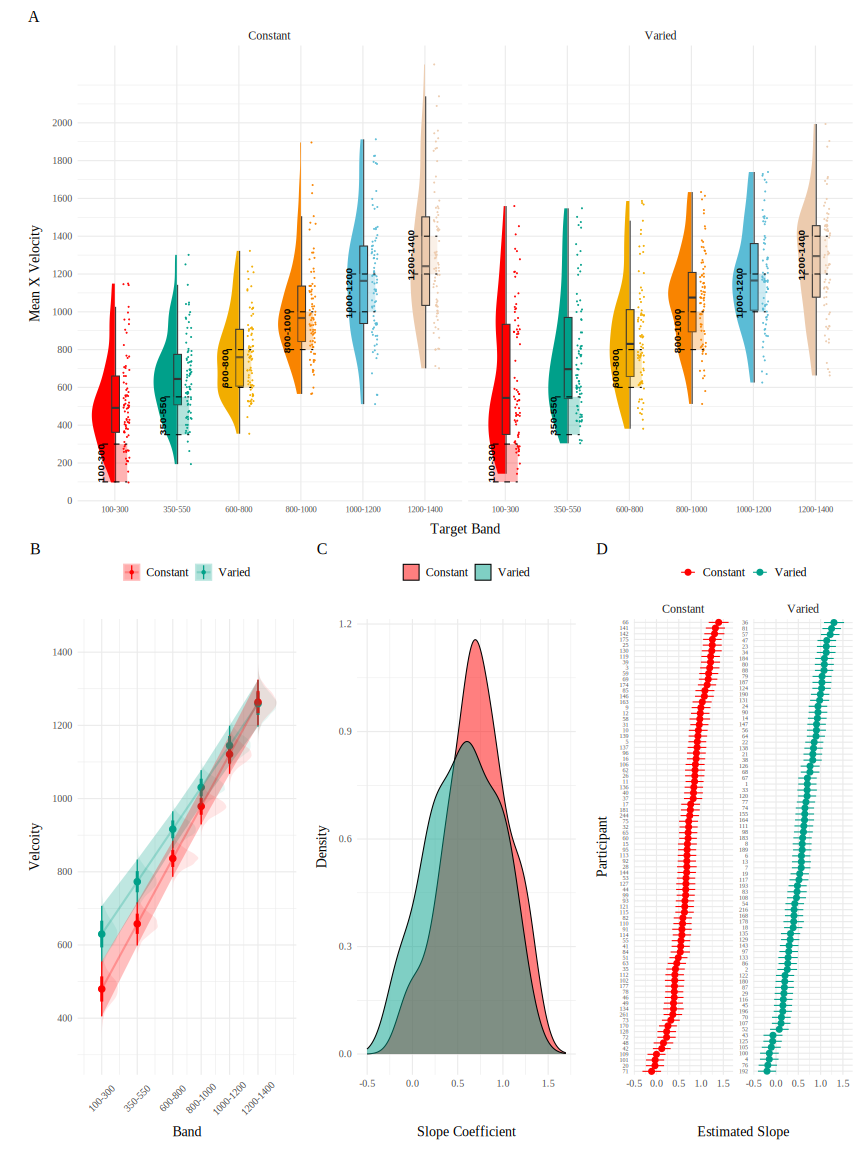
\includegraphics[width=1\textwidth,height=\textheight]{manuscript_files/figure-pdf/fig-e1-test-vx-1.pdf}

}

\caption{\label{fig-e1-test-vx}E1 testing x velocities. Translucent
bands with dash lines indicate the correct range for each velocity
band.}

\end{figure}%

\begin{table}

\caption{\label{tbl-e1-test-nf-vx}Testing vx - Empirical Summary}

\centering{

\subcaption{\label{tbl-e1-test-nf-vx-1}Constant}

\centering{

\begin{tabular}{llrrr}
\toprule
Band & Band Type & Mean & Median & Sd\\
\midrule
100-300 & Extrapolation & 524 & 448 & 327\\
350-550 & Extrapolation & 659 & 624 & 303\\
600-800 & Extrapolation & 770 & 724 & 300\\
800-1000 & Trained & 1001 & 940 & 357\\
1000-1200 & Extrapolation & 1167 & 1104 & 430\\
1200-1400 & Extrapolation & 1283 & 1225 & 483\\
\bottomrule
\end{tabular}

}

\subcaption{\label{tbl-e1-test-nf-vx-2}Varied}

\centering{

\begin{tabular}{llrrr}
\toprule
Band & Band Type & Mean & Median & Sd\\
\midrule
100-300 & Extrapolation & 664 & 533 & 448\\
350-550 & Extrapolation & 768 & 677 & 402\\
600-800 & Extrapolation & 876 & 813 & 390\\
800-1000 & Trained & 1064 & 1029 & 370\\
1000-1200 & Trained & 1180 & 1179 & 372\\
1200-1400 & Trained & 1265 & 1249 & 412\\
\bottomrule
\end{tabular}

}

}

\end{table}%

\begin{table}

\caption{\label{tbl-e1-bmm-vx}Experiment 1. Bayesian Mixed Model
Predicting Vx as a function of condition (Constant vs.~Varied) and
Velocity Band}

\centering{

\subcaption{\label{tbl-e1-bmm-vx-1}Model fit to all 6 bands}

\centering{

\begin{tabular}{lrrrr}
\toprule
Term & Estimate & 95\% CrI Lower & 95\% CrI Upper & pd\\
\midrule
Intercept & 408.55 & 327.00 & 490.61 & 1.00\\
conditVaried & 164.05 & 45.50 & 278.85 & 1.00\\
Band & 0.71 & 0.62 & 0.80 & 1.00\\
condit*Band & -0.14 & -0.26 & -0.01 & 0.98\\
\bottomrule
\end{tabular}

}

\subcaption{\label{tbl-e1-bmm-vx-2}Model fit to 3 extrapolation bands}

\centering{

\begin{tabular}{lrrrr}
\toprule
Term & Estimate & 95\% CrI Lower & 95\% CrI Upper & pd\\
\midrule
Intercept & 497.49 & 431.26 & 566.17 & 1.00\\
conditVaried & 124.79 & 26.61 & 224.75 & 0.99\\
Band & 0.49 & 0.42 & 0.56 & 1.00\\
condit*Band & -0.06 & -0.16 & 0.04 & 0.88\\
\bottomrule
\end{tabular}

}

}

\end{table}%

See Table~\ref{tbl-e1-bmm-vx} for the full model results. The estimated
coefficient for training condition (\(B\) = 164.05, 95\% CrI {[}45.5,
278.85{]}) suggests that the varied group tends to produce harder throws
than the constant group, but is not in and of itself useful for
assessing discrimination. Most relevant to the issue of discrimination
is the slope on Velocity Band (\(B\) = 0.71, 95\% CrI {[}0.62, 0.8{]}).
Although the median slope does fall underneath the ideal of value of 1,
the fact that the 95\% credible interval does not contain 0 provides
strong evidence that participants exhibited some discrimination between
bands. The estimate for the interaction between slope and condition
(\(B\) = -0.14, 95\% CrI {[}-0.26, -0.01{]}), suggests that the
discrimination was somewhat modulated by training condition, with the
varied participants showing less senitivity between vands than the
constant condition. This difference is depicted visually in
Figure~\ref{fig-e1-bmm-vx}.@tbl-e1-slope-quartile shows the average
slope coefficients for varied and constant participants separately for
each quartile. The constant participant participants appear to have
larger slopes across quartiles, but the difference between conditions
may be less pronounced for the top quartiles of subjects who show the
strongest discrimination. Figure Figure~\ref{fig-e1-bmm-bx2} shows the
distributions of slope values for each participant, and the compares the
probability density of slope coefficients between training conditions.
Figure~\ref{fig-e1-indv-slopes}

The second model, which focused solely on extrapolation bands, revealed
similar patterns. The Velocity Band term (\(B\) = 0.49, 95\% CrI
{[}0.42, 0.56{]}) still demonstrates a high degree of discrimination
ability. However, the posterior distribution for interaction term (\(B\)
= -0.06, 95\% CrI {[}-0.16, 0.04{]} ) does across over 0, suggesting
that the evidence for decreased discrimination ability for the varied
participants is not as strong when considering only the three
extrapolation bands.

\begin{figure}

\begin{minipage}{\linewidth}

\centering{

\includegraphics[width=1\textwidth,height=\textheight]{manuscript_files/figure-pdf/fig-e1-bmm-vx-1.pdf}

}

\subcaption{\label{fig-e1-bmm-vx-1}Model fit to all 6 bands}

\end{minipage}%
\newline
\begin{minipage}{\linewidth}

\centering{

\includegraphics[width=1\textwidth,height=\textheight]{manuscript_files/figure-pdf/fig-e1-bmm-vx-2.pdf}

}

\subcaption{\label{fig-e1-bmm-vx-2}Model fit to only 3 extrapolation
bands}

\end{minipage}%

\caption{\label{fig-e1-bmm-vx}Conditional effect of training condition
and Band. Ribbons indicate 95\% HDI. The steepness of the lines serves
as an indicator of how well participants discriminated between velocity
bands.}

\end{figure}%

\begin{longtable}[]{@{}lrrrrr@{}}

\caption{\label{tbl-e1-slope-quartile}Slope coefficients by quartile,
per condition}

\tabularnewline

\toprule\noalign{}
Condition & Q\_0\%\_mean & Q\_25\%\_mean & Q\_50\%\_mean & Q\_75\%\_mean
& Q\_100\%\_mean \\
\midrule\noalign{}
\endhead
\bottomrule\noalign{}
\endlastfoot
Constant & -0.109 & 0.479 & 0.691 & 0.930 & 1.39 \\
Varied & -0.202 & 0.268 & 0.588 & 0.902 & 1.30 \\

\end{longtable}

\begin{figure}

\begin{minipage}{\linewidth}

\centering{

\includegraphics[width=1\textwidth,height=\textheight]{manuscript_files/figure-pdf/fig-e1-bmm-bx2-1.pdf}

}

\subcaption{\label{fig-e1-bmm-bx2-1}Slope estimates by participant -
ordered from lowest to highest within each condition.}

\end{minipage}%
\newline
\begin{minipage}{\linewidth}

\centering{

\includegraphics[width=1\textwidth,height=\textheight]{manuscript_files/figure-pdf/fig-e1-bmm-bx2-2.pdf}

}

\subcaption{\label{fig-e1-bmm-bx2-2}Destiny of slope coefficients by
training group}

\end{minipage}%

\caption{\label{fig-e1-bmm-bx2}Slope distributions between condition}

\end{figure}%

test

\begin{figure}

\centering{

\centering{

\includegraphics[width=1\textwidth,height=\textheight]{manuscript_files/figure-pdf/fig-e1-indv-slopes-1.pdf}

}

\subcaption{\label{fig-e1-indv-slopes-1}subset with largest slopes}

\centering{

\includegraphics[width=1\textwidth,height=\textheight]{manuscript_files/figure-pdf/fig-e1-indv-slopes-2.pdf}

}

\subcaption{\label{fig-e1-indv-slopes-2}subset with smallest slopes}

}

\caption{\label{fig-e1-indv-slopes}Subset of Varied and Constant
Participants with the smallest and largest estimated slope values. Red
lines represent the best fitting line for each participant, gray lines
are 200 random samples from the posterior distribution. Colored points
and intervals at each band represent the empirical median and 95\% HDI.}

\end{figure}%

\section{Experiment 2}\label{experiment-2}

Figure~\ref{fig-design-e2} illustrates the design of Experiment 2. The
stages of the experiment (i.e.~training, testing no-feedback, test with
feedback), are identical to that of Experiment 1. The only change is
that Experiment 2 participants train, and then test, on bands in the
reverse order of Experiment 1 (i.e.~training on the softer bands; and
testing on the harder bands).

\begin{figure*}

\centering{

\includegraphics[width=6in,height=2.5in]{manuscript_files/figure-latex/dot-figure-2.png}

}

\caption{\label{fig-design-e2}Experiment 2 Design. Constant and Varied
participants complete different training conditions. The training and
testing bands are the reverse of Experiment 1.}

\end{figure*}%

\subsection{E2 Results}\label{e2-results}

\subsubsection{Testing Phase - No
feedback.}\label{testing-phase---no-feedback.-1}

In the first part of the testing phase, participants are tested from
each of the velocity bands, and receive no feedback after each throw.

\paragraph{Deviation From Target
Band}\label{deviation-from-target-band-1}

Descriptive summaries testing deviation data are provided in
Table~\ref{tbl-e2-test-nf-deviation} and Figure~\ref{fig-e2-test-dev}.
To model differences in accuracy between groups, we used Bayesian mixed
effects regression models to the trial level data from the testing
phase. The primary model predicted the absolute deviation from the
target velocity band (dist) as a function of training condition
(condit), target velocity band (band), and their interaction, with
random intercepts and slopes for each participant (id).

\begin{equation}
dist_{ij} = \beta_0 + \beta_1 \cdot condit_{ij} + \beta_2 \cdot band_{ij} + \beta_3 \cdot condit_{ij} \cdot band_{ij} + b_{0i} + b_{1i} \cdot band_{ij} + \epsilon_{ij}
\end{equation}

\begin{table}

\caption{\label{tbl-e2-test-nf-deviation}Testing Deviation - Empirical
Summary}

\centering{

\subcaption{\label{tbl-e2-test-nf-deviation-1}Constant Testing - Deviation}

\centering{

\begin{tabular}{llrrr}
\toprule
Band & Band Type & Mean & Median & Sd\\
\midrule
100-300 & Extrapolation & 206 & 48 & 317\\
350-550 & Extrapolation & 194 & 86 & 268\\
600-800 & Trained & 182 & 112 & 240\\
800-1000 & Extrapolation & 200 & 129 & 233\\
1000-1200 & Extrapolation & 238 & 190 & 234\\
1200-1400 & Extrapolation & 311 & 254 & 288\\
\bottomrule
\end{tabular}

}

\subcaption{\label{tbl-e2-test-nf-deviation-2}Varied Testing - Deviation}

\centering{

\begin{tabular}{llrrr}
\toprule
Band & Band Type & Mean & Median & Sd\\
\midrule
100-300 & Trained & 153 & 25 & 266\\
350-550 & Trained & 138 & 53 & 233\\
600-800 & Trained & 160 & 120 & 183\\
800-1000 & Extrapolation & 261 & 207 & 257\\
1000-1200 & Extrapolation & 305 & 258 & 273\\
1200-1400 & Extrapolation & 363 & 314 & 297\\
\bottomrule
\end{tabular}

}

}

\end{table}%

\begin{figure}

\centering{

\includegraphics[width=1\textwidth,height=\textheight]{manuscript_files/figure-pdf/fig-e2-test-dev-1.pdf}

}

\caption{\label{fig-e2-test-dev}E2. Deviations from target band during
testing without feedback stage.}

\end{figure}%

\begin{table}

\caption{\label{tbl-e2-bmm-dist}Experiment 2. Bayesian Mixed Model
predicting absolute deviation as a function of condition (Constant
vs.~Varied) and Velocity Band}

\centering{

\subcaption{\label{tbl-e2-bmm-dist-1}Model fits}

\centering{

\begin{tabular}{lrrrr}
\toprule
Term & Estimate & 95\% CrI Lower & 95\% CrI Upper & pd\\
\midrule
Intercept & 151.71 & 90.51 & 215.86 & 1.00\\
conditVaried & -70.33 & -156.87 & 16.66 & 0.94\\
Band & 0.10 & 0.02 & 0.18 & 1.00\\
condit*Band & 0.12 & 0.02 & 0.23 & 0.99\\
\bottomrule
\end{tabular}

}

\subcaption{\label{tbl-e2-bmm-dist-2}Contrasts}

\centering{

\begin{tabular}{lrrrrr}
\toprule
contrast & Band & value & lower & upper & pd\\
\midrule
Constant - Varied & 100 & 57.6 & -20.5 & 135.32 & 0.93\\
Constant - Varied & 350 & 26.6 & -30.9 & 83.84 & 0.83\\
Constant - Varied & 600 & -4.3 & -46.7 & 38.52 & 0.58\\
Constant - Varied & 800 & -29.3 & -69.4 & 11.29 & 0.92\\
Constant - Varied & 1000 & -54.6 & -101.1 & -5.32 & 0.98\\
Constant - Varied & 1200 & -79.6 & -139.5 & -15.45 & 0.99\\
\bottomrule
\end{tabular}

}

}

\end{table}%

The model predicting absolute deviation showed a modest tendency for the
varied training group to have lower deviation compared to the constant
training group (β = -70.33, 95\% CI {[}-156.87, 16.66{]}),with 94\% of
the posterior distribution being less than 0. This suggests a potential
benefit of training with variation, though the evidence is not
definitive.

\paragraph{Discrimination between Velocity
Bands}\label{discrimination-between-velocity-bands}

In addition to accuracy/deviation. We also assessed the ability of
participants to reliably discriminate between the velocity bands
(i.e.~responding differently when prompted for band 600-800 than when
prompted for band 150-350). Table~\ref{tbl-e2-test-nf-vx} shows
descriptive statistics of this measure, and Figure 1 visualizes the full
distributions of throws for each combination of condition and velocity
band. To quantify discrimination, we again fit Bayesian Mixed Models as
above, but this time the dependent variable was the raw x velocity
generated by participants.

\begin{equation}
vx_{ij} = \beta_0 + \beta_1 \cdot condit_{ij} + \beta_2 \cdot bandInt_{ij} + \beta_3 \cdot condit_{ij} \cdot bandInt_{ij} + b_{0i} + b_{1i} \cdot bandInt_{ij} + \epsilon_{ij}
\end{equation}

\begin{figure}

\centering{

\includegraphics[width=1\textwidth,height=\textheight]{manuscript_files/figure-pdf/fig-e2-test-vx-1.pdf}

}

\caption{\label{fig-e2-test-vx}E2 testing x velocities. Translucent
bands with dash lines indicate the correct range for each velocity
band.}

\end{figure}%

\begin{table}

\caption{\label{tbl-e2-test-nf-vx}Testing vx - Empirical Summary}

\begin{minipage}{\linewidth}

\subcaption{\label{tbl-e2-test-nf-vx-1}Constant Testing - vx}

\centering{

\begin{tabular}{llrrr}
\toprule
Band & Band Type & Mean & Median & Sd\\
\midrule
100-300 & Extrapolation & 457 & 346 & 354\\
350-550 & Extrapolation & 597 & 485 & 368\\
600-800 & Trained & 728 & 673 & 367\\
800-1000 & Extrapolation & 953 & 913 & 375\\
1000-1200 & Extrapolation & 1064 & 1012 & 408\\
1200-1400 & Extrapolation & 1213 & 1139 & 493\\
\bottomrule
\end{tabular}

}

\end{minipage}%
\newline
\begin{minipage}{\linewidth}

\subcaption{\label{tbl-e2-test-nf-vx-2}Varied Testing - vx}

\centering{

\begin{tabular}{llrrr}
\toprule
Band & Band Type & Mean & Median & Sd\\
\midrule
100-300 & Trained & 410 & 323 & 297\\
350-550 & Trained & 582 & 530 & 303\\
600-800 & Trained & 696 & 641 & 316\\
800-1000 & Extrapolation & 910 & 848 & 443\\
1000-1200 & Extrapolation & 1028 & 962 & 482\\
1200-1400 & Extrapolation & 1095 & 1051 & 510\\
\bottomrule
\end{tabular}

}

\end{minipage}%

\end{table}%

\begin{longtable}[]{@{}lrrrr@{}}

\caption{\label{tbl-e2-bmm-vx}Experiment 2. Bayesian Mixed Model
Predicting Vx as a function of condition (Constant vs.~Varied) and
Velocity Band}

\tabularnewline

\toprule\noalign{}
Term & Estimate & 95\% CrI Lower & 95\% CrI Upper & pd \\
\midrule\noalign{}
\endhead
\bottomrule\noalign{}
\endlastfoot
Intercept & 362.64 & 274.85 & 450.02 & 1.00 \\
conditVaried & -8.56 & -133.97 & 113.98 & 0.55 \\
Band & 0.71 & 0.58 & 0.84 & 1.00 \\
condit*Band & -0.06 & -0.24 & 0.13 & 0.73 \\

\end{longtable}

See Table~\ref{tbl-e2-bmm-vx} for the full model results.

When examining discrimination ability using the model predicting raw
x-velocity, the results were less clear than those of the absolute
deviation analysis. The slope on Velocity Band (β = 0.71, 95\% CrI
{[}0.58, 0.84{]}) indicates that participants showed good discrimination
between bands overall. However, the interaction term suggested this
effect was not modulated by training condition (β = -0.06, 95\% CrI
{[}-0.24, 0.13{]}) Thus, while varied training may provide some
advantage for accuracy, both training conditions seem to have similar
abilities to discriminate between velocity bands.

\begin{figure}

\centering{

\includegraphics[width=1\textwidth,height=\textheight]{manuscript_files/figure-pdf/fig-e2-bmm-vx-1.pdf}

}

\caption{\label{fig-e2-bmm-vx}Conditional effect of training condition
and Band. Ribbons indicate 95\% HDI.}

\end{figure}%

\section{Experiment 3}\label{experiment-3}

The major manipulation adjustment of experiment 3 is for participants to
receive ordinal feedback during training, in contrast to the continuous
feedback of the earlier experiments. Ordinal feedback informs
participants whether a throw was too soft, too hard, or fell within the
target velocity range. Experiment 3 participants were randomly assigned
to both a training condition (Constant vs.~Varied) and a Band Order
condition (original order used in Experiment 1, or the Reverse order of
Experiment 2).

\subsection{Results}\label{results-1}

\subsubsection{Testing Phase - No
feedback.}\label{testing-phase---no-feedback.-2}

In the first part of the testing phase, participants are tested from
each of the velocity bands, and receive no feedback after each throw.
Note that these no-feedback testing trials are identical to those of
Experiment 1 and 2, as the ordinal feedback only occurs during the
training phase, and final testing phase, of Experiment 3.

\paragraph{Deviation From Target
Band}\label{deviation-from-target-band-2}

Descriptive summaries testing deviation data are provided in
Table~\ref{tbl-e3-test-nf-deviation} and Figure~\ref{fig-e3-test-dev}.
To model differences in accuracy between groups, we fit Bayesian mixed
effects regression models to the trial level data from the testing
phase. The primary model predicted the absolute deviation from the
target velocity band (dist) as a function of training condition
(condit), target velocity band (band), and their interaction, with
random intercepts and slopes for each participant (id).

\subcaption{\label{tbl-e3-test-nf-deviation-1}Constant Testing - Deviation}

\centering{

\begin{tabular}{llrrr}
\toprule
Band & Band Type & Mean & Median & Sd\\
\midrule
100-300 & Extrapolation & 396 & 325 & 350\\
350-550 & Extrapolation & 278 & 176 & 299\\
600-800 & Extrapolation & 173 & 102 & 215\\
800-1000 & Trained & 225 & 126 & 284\\
1000-1200 & Extrapolation & 253 & 192 & 271\\
1200-1400 & Extrapolation & 277 & 210 & 262\\
\bottomrule
\end{tabular}

}

\subcaption{\label{tbl-e3-test-nf-deviation-2}Varied Testing - Deviation}

\centering{

\begin{tabular}{llrrr}
\toprule
Band & Band Type & Mean & Median & Sd\\
\midrule
100-300 & Extrapolation & 383 & 254 & 385\\
350-550 & Extrapolation & 287 & 154 & 318\\
600-800 & Extrapolation & 213 & 140 & 244\\
800-1000 & Trained & 199 & 142 & 209\\
1000-1200 & Trained & 222 & 163 & 221\\
1200-1400 & Trained & 281 & 227 & 246\\
\bottomrule
\end{tabular}

}

\begin{longtable}[]{@{}llrrr@{}}

\caption{\label{tbl-e3-test-nf-deviation}Testing Deviation - Empirical
Summary}

\tabularnewline

\toprule\noalign{}
Band & Band Type & Mean & Median & Sd \\
\midrule\noalign{}
\endhead
\bottomrule\noalign{}
\endlastfoot
100-300 & Extrapolation & 403 & 334 & 383 \\
350-550 & Extrapolation & 246 & 149 & 287 \\
600-800 & Trained & 155 & 82 & 209 \\
800-1000 & Extrapolation & 207 & 151 & 241 \\
1000-1200 & Extrapolation & 248 & 220 & 222 \\
1200-1400 & Extrapolation & 322 & 281 & 264 \\

\end{longtable}

\begin{longtable}[]{@{}llrrr@{}}

\caption{\label{tbl-e3-test-nf-deviation}Testing Deviation - Empirical
Summary}

\tabularnewline

\toprule\noalign{}
Band & Band Type & Mean & Median & Sd \\
\midrule\noalign{}
\endhead
\bottomrule\noalign{}
\endlastfoot
100-300 & Trained & 153 & 0 & 307 \\
350-550 & Trained & 147 & 55 & 258 \\
600-800 & Trained & 159 & 107 & 192 \\
800-1000 & Extrapolation & 221 & 160 & 235 \\
1000-1200 & Extrapolation & 244 & 185 & 235 \\
1200-1400 & Extrapolation & 324 & 264 & 291 \\

\end{longtable}

\begin{figure}

\centering{

\includegraphics[width=1\textwidth,height=\textheight]{manuscript_files/figure-pdf/fig-e3-test-dev-1.pdf}

}

\caption{\label{fig-e3-test-dev}e3. Deviations from target band during
testing without feedback stage.}

\end{figure}%

\begin{longtable}[]{@{}lrrrr@{}}

\caption{\label{tbl-e3-bmm-dist}Experiment 3. Bayesian Mixed Model
predicting absolute deviation as a function of condition (Constant
vs.~Varied) and Velocity Band}

\tabularnewline

\toprule\noalign{}
Term & Estimate & 95\% CrI Lower & 95\% CrI Upper & pd \\
\midrule\noalign{}
\endhead
\bottomrule\noalign{}
\endlastfoot
Intercept & 306.47 & 243.89 & 368.75 & 1.00 \\
conditVaried & -90.65 & -182.79 & 3.75 & 0.97 \\
Band & -0.07 & -0.13 & 0.00 & 0.97 \\
condit*Band & 0.09 & -0.01 & 0.19 & 0.96 \\

\end{longtable}

The effect of training condition in Experiment 3 showed a similar
pattern to Experiment 2, with the varied group tending to have lower
deviation than the constant group (β = -90.65, 95\% CrI {[}-182.79,
3.75{]}), with 97\% of the posterior distribution falling under 0.

\begin{figure}

\centering{

\includegraphics[width=1\textwidth,height=\textheight]{manuscript_files/figure-pdf/fig-e3-bmm-dist-1.pdf}

}

\caption{\label{fig-e3-bmm-dist}e3. Conditioinal Effect of Training
Condition and Band. Ribbon indicated 95\% Credible Intervals.}

\end{figure}%

\paragraph{Discrimination between Velocity
Bands}\label{discrimination-between-velocity-bands-1}

In addition to accuracy/deviation. We also assessed the ability of
participants to reliably discriminate between the velocity bands
(i.e.~responding differently when prompted for band 600-800 than when
prompted for band 150-350). Table~\ref{tbl-e3-test-nf-vx} shows
descriptive statistics of this measure, and Figure 1 visualizes the full
distributions of throws for each combination of condition and velocity
band. To quantify discrimination, we again fit Bayesian Mixed Models as
above, but this time the dependent variable was the raw x velocity
generated by participants.

\begin{equation}
vx_{ij} = \beta_0 + \beta_1 \cdot condit_{ij} + \beta_2 \cdot bandInt_{ij} + \beta_3 \cdot condit_{ij} \cdot bandInt_{ij} + b_{0i} + b_{1i} \cdot bandInt_{ij} + \epsilon_{ij}
\end{equation}

\begin{figure}

\centering{

\includegraphics[width=1\textwidth,height=\textheight]{manuscript_files/figure-pdf/fig-e3-test-vx-1.pdf}

}

\caption{\label{fig-e3-test-vx}e3 testing x velocities. Translucent
bands with dash lines indicate the correct range for each velocity
band.}

\end{figure}%

\subcaption{\label{tbl-e3-test-nf-vx-1}Constant Testing - vx}

\centering{

\begin{tabular}{llrrr}
\toprule
Band & Band Type & Mean & Median & Sd\\
\midrule
100-300 & Extrapolation & 680 & 625 & 370\\
350-550 & Extrapolation & 771 & 716 & 357\\
600-800 & Extrapolation & 832 & 786 & 318\\
800-1000 & Trained & 1006 & 916 & 417\\
1000-1200 & Extrapolation & 1149 & 1105 & 441\\
1200-1400 & Extrapolation & 1180 & 1112 & 443\\
\bottomrule
\end{tabular}

}

\subcaption{\label{tbl-e3-test-nf-vx-2}Varied Testing - vx}

\centering{

\begin{tabular}{llrrr}
\toprule
Band & Band Type & Mean & Median & Sd\\
\midrule
100-300 & Extrapolation & 667 & 554 & 403\\
350-550 & Extrapolation & 770 & 688 & 383\\
600-800 & Extrapolation & 869 & 814 & 358\\
800-1000 & Trained & 953 & 928 & 359\\
1000-1200 & Trained & 1072 & 1066 & 388\\
1200-1400 & Trained & 1144 & 1093 & 426\\
\bottomrule
\end{tabular}

}

\begin{longtable}[]{@{}llrrr@{}}

\caption{\label{tbl-e3-test-nf-vx}Testing vx - Empirical Summary}

\tabularnewline

\toprule\noalign{}
Band & Band Type & Mean & Median & Sd \\
\midrule\noalign{}
\endhead
\bottomrule\noalign{}
\endlastfoot
100-300 & Extrapolation & 684 & 634 & 406 \\
350-550 & Extrapolation & 729 & 679 & 350 \\
600-800 & Trained & 776 & 721 & 318 \\
800-1000 & Extrapolation & 941 & 883 & 387 \\
1000-1200 & Extrapolation & 1014 & 956 & 403 \\
1200-1400 & Extrapolation & 1072 & 1014 & 442 \\

\end{longtable}

\begin{longtable}[]{@{}llrrr@{}}

\caption{\label{tbl-e3-test-nf-vx}Testing vx - Empirical Summary}

\tabularnewline

\toprule\noalign{}
Band & Band Type & Mean & Median & Sd \\
\midrule\noalign{}
\endhead
\bottomrule\noalign{}
\endlastfoot
100-300 & Trained & 392 & 270 & 343 \\
350-550 & Trained & 540 & 442 & 343 \\
600-800 & Trained & 642 & 588 & 315 \\
800-1000 & Extrapolation & 943 & 899 & 394 \\
1000-1200 & Extrapolation & 1081 & 1048 & 415 \\
1200-1400 & Extrapolation & 1185 & 1129 & 500 \\

\end{longtable}

\begin{longtable}[]{@{}lrrrr@{}}

\caption{\label{tbl-e3-bmm-vx}Experiment 3. Bayesian Mixed Model
Predicting Vx as a function of condition (Constant vs.~Varied) and
Velocity Band}

\tabularnewline

\toprule\noalign{}
Term & Estimate & 95\% CrI Lower & 95\% CrI Upper & pd \\
\midrule\noalign{}
\endhead
\bottomrule\noalign{}
\endlastfoot
Intercept & 607.67 & 536.02 & 679.87 & 1 \\
conditVaried & -167.76 & -277.14 & -64.08 & 1 \\
Band & 0.44 & 0.35 & 0.52 & 1 \\
condit*Band & 0.18 & 0.06 & 0.31 & 1 \\

\end{longtable}

See Table~\ref{tbl-e3-bmm-vx} for the full model results.

Slope estimates for experiment 3 suggest that participants were capable
of distinguishing between velocity bands even when provided only ordinal
feedback during training (β = 0.44, 95\% CrI {[}0.35, 0.52{]}). Unlike
the previous two experiments, the posterior distribution for the
interaction between condition and band was consistently positive,
suggestive of superior discrimination for the varied participants β =
0.18, 95\% CrI {[}0.06, 0.31{]}.

\subsubsection{Computational Modelling}\label{computational-modelling}

\begin{figure}

\centering{

\includegraphics[width=1\textwidth,height=\textheight]{manuscript_files/figure-pdf/fig-alm-diagram-1.pdf}

}

\caption{\label{fig-alm-diagram}The basic structure of the ALM model.}

\end{figure}%

\newpage{}

\section{Modeling Approach}\label{modeling-approach}

In project 1, I applied model-based techniques to quantify and control
for the similarity between training and testing experience, which in
turn enabled us to account for the difference between varied and
constant training via an extended version of a similarity based
generalization model. In project 2, I will go a step further,
implementing a full process model capable of both 1) producing novel
responses and 2) modeling behavior in both the learning and testing
stages of the experiment. For this purpose, we will apply the
associative learning model (ALM) and the EXAM model of function learning
(\citeproc{ref-deloshExtrapolationSineQua1997}{DeLosh et al., 1997}).
ALM is a simple connectionist learning model which closely resembles
Kruschke's ALCOVE model
(\citeproc{ref-kruschkeALCOVEExemplarbasedConnectionist1992}{Kruschke,
1992}), with modifications to allow for the generation of continuous
responses.

\subsection{ALM \& Exam Description}\label{alm-exam-description}

ALM is a localist neural network model
(\citeproc{ref-pageConnectionistModellingPsychology2000a}{Page, 2000}),
with each input node corresponding to a particular stimulus, and each
output node corresponding to a particular response value. The units in
the input layer activate as a function of their Gaussian similarity to
the input stimulus. So, for example, an input stimulus of value 55 would
induce maximal activation of the input unit tuned to 55. Depending on
the value of the generalization parameter, the nearby units (e.g.~54 and
56; 53 and 57) may also activate to some degree. ALM is structured with
input and output nodes that correspond to regions of the stimulus space,
and response space, respectively. The units in the input layer activate
as a function of their similarity to a presented stimulus. As was the
case with the exemplar-based models, similarity in ALM is exponentially
decaying function of distance. The input layer is fully connected to the
output layer, and the activation for any particular output node is
simply the weighted sum of the connection weights between that node and
the input activations. The network then produces a response by taking
the weighted average of the output units (recall that each output unit
has a value corresponding to a particular response). During training,
the network receives feedback which activates each output unit as a
function of its distance from the ideal level of activation necessary to
produce the correct response. The connection weights between input and
output units are then updated via the standard delta learning rule,
where the magnitude of weight changes are controlled by a learning rate
parameter. The EXAM model is an extension of ALM, with the same learning
rule and representational scheme for input and output units. The primary
difference is that EXAM includes a linear extrapolation mechanism for
generating novel responses during testing, a modification necessary to
account for human extrapolation patterns in past research Brown \&
Lacroix (\citeproc{ref-brownUnderestimationLinearFunction2017}{2017}).
Although this extrapolation rule departs from a strictly
similarity-based generalization mechanism, EXAM is distinct from pure
rule-based models in that it remains constrained by the weights learned
during training.

See Table~\ref{tbl-alm-exam} for a full specification of the equations
that define ALM and EXAM.

\begin{figure*}

\begin{longtable}[]{@{}
  >{\raggedright\arraybackslash}p{(\columnwidth - 4\tabcolsep) * \real{0.2466}}
  >{\raggedright\arraybackslash}p{(\columnwidth - 4\tabcolsep) * \real{0.4110}}
  >{\raggedright\arraybackslash}p{(\columnwidth - 4\tabcolsep) * \real{0.3425}}@{}}
\caption{ALM \& EXAM Equations}\label{tbl-alm-exam}\tabularnewline
\toprule\noalign{}
\begin{minipage}[b]{\linewidth}\raggedright
\end{minipage} & \begin{minipage}[b]{\linewidth}\raggedright
\textbf{ALM Response Generation}
\end{minipage} & \begin{minipage}[b]{\linewidth}\raggedright
\end{minipage} \\
\midrule\noalign{}
\endfirsthead
\toprule\noalign{}
\begin{minipage}[b]{\linewidth}\raggedright
\end{minipage} & \begin{minipage}[b]{\linewidth}\raggedright
\textbf{ALM Response Generation}
\end{minipage} & \begin{minipage}[b]{\linewidth}\raggedright
\end{minipage} \\
\midrule\noalign{}
\endhead
\bottomrule\noalign{}
\endlastfoot
Input Activation &
\(a_i(X) = \frac{e^{-c(X-X_i)^2}}{\sum_{k=1}^M e^{-c(X-X_k)^2}}\) &
Input nodes activate as a function of Gaussian similarity to stimulus \\
Output Activation & \(O_j(X) = \sum_{k=1}^M w_{ji} \cdot a_i(X)\) &
Output unit \(O_j\) activation is the weighted sum of input activations
and association weights \\
Output Probability & \(P[Y_j|X] = \frac{O_j(X)}{\sum_{k=1}^M O_k(X)}\) &
The response, \(Y_j\) probabilites computed via Luce's choice rule \\
Mean Output &
\(m(X) = \sum_{j=1}^L Y_j \cdot \frac{O_j(x)}{\sum_{k=1}^M O_k(X)}\) &
Weighted average of probabilities determines response to X \\
& \textbf{ALM Learning} & \\
Feedback & \(f_j(Z) = e^{-c(Z-Y_j)^2}\) & feedback signal Z computed as
similarity between ideal response and observed response \\
magnitude of error & \(\Delta_{ji}=(f_{j}(Z)-o_{j}(X))a_{i}(X)\) & Delta
rule to update weights. \\
Update Weights & \(w_{ji}^{new}=w_{ji}+\eta\Delta_{ji}\) & Updates
scaled by learning rate parameter \(\eta\). \\
& \textbf{EXAM Extrapolation} & \\
Instance Retrieval & \(P[X_i|X] = \frac{a_i(X)}{\sum_{k=1}^M a_k(X)}\) &
Novel test stimulus \(X\) activates input nodes \(X_i\) \\
Slope Computation & \(S =\) \(\frac{m(X_{1})-m(X_{2})}{X_{1}-X_{2}}\) &
Slope value, \(S\) computed from nearest training instances \\
Response & \(E[Y|X_i] = m(X_i) + S \cdot [X - X_i]\) & ALM response
\(m(X_i)\) adjusted by slope. \\
\end{longtable}

\end{figure*}%

\subsection{Model Fitting Strategy}\label{model-fitting-strategy}

To fit ALM and EXAM to our participant data, we employ a similar method
to Mcdaniel et al.
(\citeproc{ref-mcdanielPredictingTransferPerformance2009}{2009}),
wherein we examine the performance of each model after being fit to
various subsets of the data. Each model was fit to the data in with
separate procedures: 1) fit to maximize predictions of the testing data,
2) fit to maximize predictions of both the training and testing data, 3)
fit to maximize predictions of the just the training data. We refer to
this fitting manipulations as ``Fit Method'' in the tables and figures
below. It should be emphasized that for all three fit methods, the ALM
and EXAM models behave identically - with weights updating only during
the training phase.Models to were fit separately to the data of each
individual participant. The free parameters for both models are the
generalization (\(c\)) and learning rate (\(lr\)) parameters. Parameter
estimation was performed using approximate bayesian computation (ABC),
which we describe in detail below.

\subsubsection{Approximate Bayesian
Computation}\label{approximate-bayesian-computation}

To estimate parameters, we used approximate bayesian computation (ABC),
enabling us to obtain an estimate of the posterior distribution of the
generalization and learning rate parameters for each individual. ABC
belongs to the class of simulation-based inference methods
(\citeproc{ref-cranmerFrontierSimulationbasedInference2020}{Cranmer et
al., 2020}), which have begun being used for parameter estimation in
cognitive modeling relatively recently
(\citeproc{ref-kangasraasioParameterInferenceComputational2019}{Kangasrääsiö
et al., 2019};
\citeproc{ref-turnerBayesianAnalysisSimulationbased2016}{Turner et al.,
2016}; \citeproc{ref-turnerTutorialApproximateBayesian2012}{Turner \&
Van Zandt, 2012}). Although they can be applied to any model from which
data can be simulated, ABC methods are most useful for complex models
that lack an explicit likelihood function (e.g.~many neural network and
evidence accumulation models).

The general ABC procedure is to 1) define a prior distribution over
model parameters. 2) sample candidate parameter values, \(\theta^*\),
from the prior. 3) Use \(\theta^*\) to generate a simulated dataset,
\(Data_{sim}\). 4) Compute a measure of discrepancy between the
simulated and observed datasets, \(discrep\)(\(Data_{sim}\),
\(Data_{obs}\)). 5) Accept \(\theta^*\) if the discrepancy is less than
the tolerance threshold, \(\epsilon\), otherwise reject \(\theta^*\). 6)
Repeat until desired number of posterior samples are obtained.

Although simple in the abstract, implementations of ABC require
researchers to make a number of non-trivial decisions as to i) the
discrepancy function between observed and simulated data, ii) whether to
compute the discrepancy between trial level data, or a summary statistic
of the datasets, iii) the value of the minimum tolerance \(\epsilon\).
For the present work, we follow the guidelines from published ABC
tutorials
(\citeproc{ref-farrellComputationalModelingCognition2018}{Farrell \&
Lewandowsky, 2018};
\citeproc{ref-turnerTutorialApproximateBayesian2012}{Turner \& Van
Zandt, 2012}). For the test stage, we summarized datasets with mean
velocity of each band in the observed dataset as \(V_{obs}^{(k)}\) and
in the simulated dataset as \(V_{sim}^{(k)}\), where
\(k \in \{1, 2, 3, 4, 5, 6\}\) represents each of the six velocity
bands. For computing the discrepancy between datasets in the training
stage, we aggregated training trials into three equally sized blocks
(separately for each velocity band in the case of the varied group).
After obtaining the summary statistics of the simulated and observed
datasets, the discrepancy was computed as the mean of the absolute
difference between simulated and observed datasets
(Equation~\ref{eq-discrep-test} and Equation~\ref{eq-discrep-train}).

\begin{equation}\phantomsection\label{eq-discrep-test}{
discrep_{Test}(Data_{sim}, Data_{obs}) = \frac{1}{6} \sum_{k=1}^{6} |V_{obs}^{(k)} - V_{sim}^{(k)}|
}\end{equation}

\begin{equation}\phantomsection\label{eq-discrep-train}{
\begin{aligned} \\
discrep_{Train,constant}(Data_{sim}, Data_{obs}) = \frac{1}{N_{blocks}} \sum_{j=1}^{N_{blocks}} |V_{obs,constant}^{(j)} - V_{sim,constant}^{(j)}| \\ \\
discrep_{Train,varied}(Data_{sim}, Data_{obs}) = \frac{1}{N_{blocks} \times 3} \sum_{j=1}^{N_{blocks}} \sum_{k=1}^{3} |V_{obs,varied}^{(j,k)} - V_{sim,varied}^{(j,k)}|
\end{aligned}
}\end{equation}

The final component of our ABC implementation is the determination the
appropriate value of \(\epsilon\). The setting of \(\epsilon\) exerts
strong influence on the approximated posterior distribution. Smaller
values of \(\epsilon\) increase the rejection rate, and improve the
fidelity of the approximated posterior, while larger values result in an
ABC sampler that reproduces the prior distribution. Because the
individual participants in our dataset differed substantially in terms
of the noisiness of their data, we employed an adaptive tolerance
setting strategy to tailor \(\epsilon\) to each individual. The initial
value of \(\epsilon\) was set to the overall standard deviation of each
individuals velocity values. Thus, sampled parameter values that
generated simulated data within a standard deviation of the observed
data were accepted, while worse performing parameters were rejected.
After every 300 samples the tolerance was allowed to increase only if
the current acceptance rate of the algorithm was less than 1\%. In such
cases, the tolerance was shifted towards the average discrepancy of the
5 best samples obtained thus far. To ensure the acceptance rate did not
become overly permissive, \(\epsilon\) was also allowed to decrease
every time a sample was accepted into the posterior.

For each of the 156 participants from Experiment 1, the ABC algorithm
was run until 200 samples of parameters were accepted into the posterior
distribution. Obtaining this number of posterior samples required an
average of 205,000 simulation runs per participant. Fitting each
combination of participant, Model (EXAM \& ALM), and fitting method
(Test only, Train only, Test \& Train) required a total of 192 million
simulation runs. To facilitate these intensive computational demands, we
used the Future Package in R
(\citeproc{ref-bengtssonUnifyingFrameworkParallel2021}{Bengtsson,
2021}), allowing us to parallelize computations across a cluster of ten
M1 iMacs, each with 8 cores.

\subsubsection{Modelling Results}\label{modelling-results}

\subsubsection{Group level fits}\label{group-level-fits}

\global\setlength{\Oldarrayrulewidth}{\arrayrulewidth}

\global\setlength{\Oldtabcolsep}{\tabcolsep}

\setlength{\tabcolsep}{0pt}

\renewcommand*{\arraystretch}{1.5}



\providecommand{\ascline}[3]{\noalign{\global\arrayrulewidth #1}\arrayrulecolor[HTML]{#2}\cline{#3}}

\begin{longtable}[c]{|p{1.03in}|p{0.70in}|p{0.08in}|p{0.88in}|p{0.08in}|p{0.71in}}

\caption{\label{tbl-htw-modelError}Mean model errors predicting testing
data, aggregated over all participants and velocity bands. Note that Fit
Method refers to how model parameters were optimized, while error values
reflect mean absolute error for the 6 testing bands}

\tabularnewline

\ascline{1.5pt}{666666}{1-2}\ascline{1.5pt}{666666}{4-4}\ascline{1.5pt}{666666}{6-6}

\multicolumn{1}{>{\raggedright}b{\dimexpr 1.03in+0\tabcolsep}}{\textcolor[HTML]{000000}{\fontsize{11}{11}\selectfont{Fit\_Method}}} & \multicolumn{1}{>{\raggedright}b{\dimexpr 0.7in+0\tabcolsep}}{\textcolor[HTML]{000000}{\fontsize{11}{11}\selectfont{Model}}} & \multicolumn{1}{>{\raggedright}m{\dimexpr 0.08in+0\tabcolsep}}{\textcolor[HTML]{000000}{\fontsize{11}{11}\selectfont{}}} & \multicolumn{1}{>{\centering}m{\dimexpr 0.88in+0\tabcolsep}}{\textcolor[HTML]{000000}{\fontsize{11}{11}\selectfont{Constant}}} & \multicolumn{1}{>{\raggedright}m{\dimexpr 0.08in+0\tabcolsep}}{\textcolor[HTML]{000000}{\fontsize{11}{11}\selectfont{}}} & \multicolumn{1}{>{\centering}m{\dimexpr 0.71in+0\tabcolsep}}{\textcolor[HTML]{000000}{\fontsize{11}{11}\selectfont{Varied}}} \\

\ascline{1.5pt}{666666}{1-2}\ascline{1.5pt}{666666}{4-4}\ascline{1.5pt}{666666}{6-6}\endfirsthead 

\ascline{1.5pt}{666666}{1-2}\ascline{1.5pt}{666666}{4-4}\ascline{1.5pt}{666666}{6-6}

\multicolumn{1}{>{\raggedright}b{\dimexpr 1.03in+0\tabcolsep}}{\textcolor[HTML]{000000}{\fontsize{11}{11}\selectfont{Fit\_Method}}} & \multicolumn{1}{>{\raggedright}b{\dimexpr 0.7in+0\tabcolsep}}{\textcolor[HTML]{000000}{\fontsize{11}{11}\selectfont{Model}}} & \multicolumn{1}{>{\raggedright}m{\dimexpr 0.08in+0\tabcolsep}}{\textcolor[HTML]{000000}{\fontsize{11}{11}\selectfont{}}} & \multicolumn{1}{>{\centering}m{\dimexpr 0.88in+0\tabcolsep}}{\textcolor[HTML]{000000}{\fontsize{11}{11}\selectfont{Constant}}} & \multicolumn{1}{>{\raggedright}m{\dimexpr 0.08in+0\tabcolsep}}{\textcolor[HTML]{000000}{\fontsize{11}{11}\selectfont{}}} & \multicolumn{1}{>{\centering}m{\dimexpr 0.71in+0\tabcolsep}}{\textcolor[HTML]{000000}{\fontsize{11}{11}\selectfont{Varied}}} \\

\ascline{1.5pt}{666666}{1-2}\ascline{1.5pt}{666666}{4-4}\ascline{1.5pt}{666666}{6-6}\endhead



\multicolumn{1}{>{\raggedright}p{\dimexpr 1.03in+0\tabcolsep}}{} & \multicolumn{1}{>{\raggedright}p{\dimexpr 0.7in+0\tabcolsep}}{\textcolor[HTML]{000000}{\fontsize{11}{11}\selectfont{ALM}}} & \multicolumn{1}{>{\raggedright}p{\dimexpr 0.08in+0\tabcolsep}}{\textcolor[HTML]{000000}{\fontsize{11}{11}\selectfont{}}} & \multicolumn{1}{>{\centering}p{\dimexpr 0.88in+0\tabcolsep}}{\textcolor[HTML]{000000}{\fontsize{11}{11}\selectfont{276.7}}} & \multicolumn{1}{>{\raggedright}p{\dimexpr 0.08in+0\tabcolsep}}{\textcolor[HTML]{000000}{\fontsize{11}{11}\selectfont{}}} & \multicolumn{1}{>{\centering}p{\dimexpr 0.71in+0\tabcolsep}}{\textcolor[HTML]{000000}{\fontsize{11}{11}\selectfont{231.2}}} \\





\multicolumn{1}{>{\raggedright}p{\dimexpr 1.03in+0\tabcolsep}}{\multirow[t]{-2}{*}{\parbox{1.03in}{\raggedright \textcolor[HTML]{000000}{\fontsize{11}{11}\selectfont{Test}}}}} & \multicolumn{1}{>{\raggedright}p{\dimexpr 0.7in+0\tabcolsep}}{\textcolor[HTML]{000000}{\fontsize{11}{11}\selectfont{EXAM}}} & \multicolumn{1}{>{\raggedright}p{\dimexpr 0.08in+0\tabcolsep}}{\textcolor[HTML]{000000}{\fontsize{11}{11}\selectfont{}}} & \multicolumn{1}{>{\centering}p{\dimexpr 0.88in+0\tabcolsep}}{\textcolor[HTML]{000000}{\fontsize{11}{11}\selectfont{215.9}}} & \multicolumn{1}{>{\raggedright}p{\dimexpr 0.08in+0\tabcolsep}}{\textcolor[HTML]{000000}{\fontsize{11}{11}\selectfont{}}} & \multicolumn{1}{>{\centering}p{\dimexpr 0.71in+0\tabcolsep}}{\textcolor[HTML]{000000}{\fontsize{11}{11}\selectfont{215.0}}} \\





\multicolumn{1}{>{\raggedright}p{\dimexpr 1.03in+0\tabcolsep}}{} & \multicolumn{1}{>{\raggedright}p{\dimexpr 0.7in+0\tabcolsep}}{\textcolor[HTML]{000000}{\fontsize{11}{11}\selectfont{ALM}}} & \multicolumn{1}{>{\raggedright}p{\dimexpr 0.08in+0\tabcolsep}}{\textcolor[HTML]{000000}{\fontsize{11}{11}\selectfont{}}} & \multicolumn{1}{>{\centering}p{\dimexpr 0.88in+0\tabcolsep}}{\textcolor[HTML]{000000}{\fontsize{11}{11}\selectfont{288.2}}} & \multicolumn{1}{>{\raggedright}p{\dimexpr 0.08in+0\tabcolsep}}{\textcolor[HTML]{000000}{\fontsize{11}{11}\selectfont{}}} & \multicolumn{1}{>{\centering}p{\dimexpr 0.71in+0\tabcolsep}}{\textcolor[HTML]{000000}{\fontsize{11}{11}\selectfont{268.3}}} \\





\multicolumn{1}{>{\raggedright}p{\dimexpr 1.03in+0\tabcolsep}}{\multirow[t]{-2}{*}{\parbox{1.03in}{\raggedright \textcolor[HTML]{000000}{\fontsize{11}{11}\selectfont{Test\_Train}}}}} & \multicolumn{1}{>{\raggedright}p{\dimexpr 0.7in+0\tabcolsep}}{\textcolor[HTML]{000000}{\fontsize{11}{11}\selectfont{EXAM}}} & \multicolumn{1}{>{\raggedright}p{\dimexpr 0.08in+0\tabcolsep}}{\textcolor[HTML]{000000}{\fontsize{11}{11}\selectfont{}}} & \multicolumn{1}{>{\centering}p{\dimexpr 0.88in+0\tabcolsep}}{\textcolor[HTML]{000000}{\fontsize{11}{11}\selectfont{228.6}}} & \multicolumn{1}{>{\raggedright}p{\dimexpr 0.08in+0\tabcolsep}}{\textcolor[HTML]{000000}{\fontsize{11}{11}\selectfont{}}} & \multicolumn{1}{>{\centering}p{\dimexpr 0.71in+0\tabcolsep}}{\textcolor[HTML]{000000}{\fontsize{11}{11}\selectfont{250.7}}} \\





\multicolumn{1}{>{\raggedright}p{\dimexpr 1.03in+0\tabcolsep}}{} & \multicolumn{1}{>{\raggedright}p{\dimexpr 0.7in+0\tabcolsep}}{\textcolor[HTML]{000000}{\fontsize{11}{11}\selectfont{ALM}}} & \multicolumn{1}{>{\raggedright}p{\dimexpr 0.08in+0\tabcolsep}}{\textcolor[HTML]{000000}{\fontsize{11}{11}\selectfont{}}} & \multicolumn{1}{>{\centering}p{\dimexpr 0.88in+0\tabcolsep}}{\textcolor[HTML]{000000}{\fontsize{11}{11}\selectfont{528.1}}} & \multicolumn{1}{>{\raggedright}p{\dimexpr 0.08in+0\tabcolsep}}{\textcolor[HTML]{000000}{\fontsize{11}{11}\selectfont{}}} & \multicolumn{1}{>{\centering}p{\dimexpr 0.71in+0\tabcolsep}}{\textcolor[HTML]{000000}{\fontsize{11}{11}\selectfont{368.7}}} \\





\multicolumn{1}{>{\raggedright}p{\dimexpr 1.03in+0\tabcolsep}}{\multirow[t]{-2}{*}{\parbox{1.03in}{\raggedright \textcolor[HTML]{000000}{\fontsize{11}{11}\selectfont{Train}}}}} & \multicolumn{1}{>{\raggedright}p{\dimexpr 0.7in+0\tabcolsep}}{\textcolor[HTML]{000000}{\fontsize{11}{11}\selectfont{EXAM}}} & \multicolumn{1}{>{\raggedright}p{\dimexpr 0.08in+0\tabcolsep}}{\textcolor[HTML]{000000}{\fontsize{11}{11}\selectfont{}}} & \multicolumn{1}{>{\centering}p{\dimexpr 0.88in+0\tabcolsep}}{\textcolor[HTML]{000000}{\fontsize{11}{11}\selectfont{340.3}}} & \multicolumn{1}{>{\raggedright}p{\dimexpr 0.08in+0\tabcolsep}}{\textcolor[HTML]{000000}{\fontsize{11}{11}\selectfont{}}} & \multicolumn{1}{>{\centering}p{\dimexpr 0.71in+0\tabcolsep}}{\textcolor[HTML]{000000}{\fontsize{11}{11}\selectfont{370.9}}} \\

\ascline{1.5pt}{666666}{1-2}\ascline{1.5pt}{666666}{4-4}\ascline{1.5pt}{666666}{6-6}


\end{longtable}

\arrayrulecolor[HTML]{000000}

\global\setlength{\arrayrulewidth}{\Oldarrayrulewidth}

\global\setlength{\tabcolsep}{\Oldtabcolsep}

\renewcommand*{\arraystretch}{1}

The posterior distributions of the \(c\) and \(lr\) parameters are shown
Figure~\ref{fig-htw-post-dist} (i.e.~these plots combine all the
posterior samples from all of the subjects). There were substantial
individual differences in the posteriors of both parameters, with the
within-group individual differences generally swamped any between-group
or between-model differences. The magnitude of these individual
differences remains even if we consider only the single best parameter
set for each subject.

We used the posterior distribution of \(c\) and \(lr\) parameters to
generate a posterior predictive distribution of the observed data for
each participant, which then allows us to compare the empirical data to
the full range of predictions from each model. Model residuals are shown
in the upper panels of Figure~\ref{fig-htw-resid-pred}. The pattern of
training stage residual errors are unsurprising across the combinations
of models and fitting method . Differences between ALM and EXAM are
generally minor (the two models have identical learning mechanisms). The
differences in the magnitude of residuals across the three fitting
methods are also straightforward, with massive errors for the `fit to
Test Only' model, and the smallest errors for the `fit to train only'
models. It is also noteworthy that the residual errors are generally
larger for the first block of training, which is likely due to the
initial values of the ALM weights being unconstrained by whatever
initial biases participants tend to bring to the task. Future work may
explore the ability of the models to capture more fine grained aspects
of the learning trajectories. However for the present purposes, our
primary interest is in the ability of ALM and EXAM to account for the
testing patterns while being constrained, or not constrained, by the
training data. All subsequent analyses and discussion will thus focus on
the testing stage.

The residuals of model predictions for the testing stage
(Figure~\ref{fig-htw-resid-pred}) show the opposite pattern of fitting
method - with models fit only to the test data showing the best
performance, followed by models fit to both training and test data, and
with models fit only to the training data showing the worst performance
(note that y axes are scaled different between plots). Unsurprisingly,
the advantage of EXAM is strongest for extrapolation positions (the
three smallest bands for both groups - as well as the two highest bands
for the Constant group). Although EXAM tends to perform better for both
Constant and Varied participants (see also
Table~\ref{tbl-htw-modelError}), the relative advantage of EXAM is
generally larger for the Constant group - a pattern consistent across
all three fitting methods. Panel B of Figure~\ref{fig-htw-resid-pred}
directly compares the aggregated observed data to the posterior
predictive distributions for the testing stage. Of interest are a) the
extent to which the median estimates of the ALM and EXAM posteriors
deviate from the observed medians for each velocity band; b) the ability
of ALM and EXAM to discriminate between velocity bands; c) the relative
performance of models that are constrained by the training data
(i.e.~the `fit to train only' and `fit to both' models) compared to the
`fit to test only' models; and d) the extent to which the variance of
the posterior predictive distributions mimics the variance of the
observed data.

\begin{itemize}
\item
  ** explain how the constant group ALM predictions for band 100 look
  deceptively good due to aggregation of a large subset of subjects
  having ALM predictions of 0 for vb100, and a large subset with ALM
  predictions close to their position 800 value. This is relected by
  much greater variance of the ALM esimates in the posterior predictive
  plot
\item
  ** comment on how much constrained by the training data has a worse
  impact on the EXAM predictions for varied than for constant - perhaps
  due to the varied training data being much noisier than the constant
  training data.
\item
  ** comment on EXAM doing a better job mimicing the within-condition
  variance of the observed data
\item
  ** comment on the \% of Constant subjects being best accounted for by
  EXAM being higher.
\end{itemize}

\begin{figure*}

\centering{

\includegraphics[width=1\textwidth,height=\textheight]{manuscript_files/figure-pdf/fig-htw-resid-pred-1.pdf}

}

\caption{\label{fig-htw-resid-pred}A) Model residuals for each
combination of training condition, fit method, and model. Residuals
reflect the difference between observed and predicted values. Lower
values indicate better model fit. Note that y axes are scaled
differently between facets. B) Full posterior predictive distributions
vs.~observed data from participants.Points represent median values,
thicker intervals represent 66\% credible intervals and thin intervals
represent 95\% credible intervals around the median.}

\end{figure*}%

\begin{figure}

\centering{

\includegraphics[width=1\textwidth,height=\textheight]{manuscript_files/figure-pdf/fig-htw-post-dist-1.pdf}

}

\caption{\label{fig-htw-post-dist}Posterior Distributions of \(c\) and
\(lr\) parameters. Points represent median values, thicker intervals
represent 66\% credible intervals and thin intervals represent 95\%
credible intervals around the median. Note that the y axes of the plots
for the c parameter are scaled logarithmically.}

\end{figure}%

To more accurately assess the relative abilities of ALM and EXAM to
capture important empirical patterns - we will now examine the
predictions of both models for the subset of individual participants
shown in Figure~\ref{fig-htw-indv-pred}. Panel A presents three varied
and constant participants who demonstrated a reasonable degree of
discrimination between the 6 velocity bands during testing.

\begin{itemize}
\item
  ** comment on the different ways ALM can completely fail to mimic
  discrimination patterns (sbj. 35; sbj. 137),and on how it can
  sometimes partially succeed (sbj. 11; 14,74)
\item
  ** comment on how EXAM can somtimes mimic non-monotonic spacing
  between bands due to associative stregth from training (i.e.~subject
  47)
\item
  ** compare c values to slope parameters from the statistical models
  earlier in paper
\end{itemize}

\begin{figure}

\centering{

\includegraphics[width=1\textwidth,height=\textheight]{manuscript_files/figure-pdf/fig-htw-indv-pred-1.pdf}

}

\caption{\label{fig-htw-indv-pred}Model predictions alongside observed
data for a subset of individual participants. A) 3 constant and 3 varied
participants fit to both the test and training data. B) 3 constant and 3
varied subjects fit to only the trainign data.}

\end{figure}%

\subsubsection{To add to appendix}\label{to-add-to-appendix}

\global\setlength{\Oldarrayrulewidth}{\arrayrulewidth}

\global\setlength{\Oldtabcolsep}{\tabcolsep}

\setlength{\tabcolsep}{0pt}

\renewcommand*{\arraystretch}{1.5}



\providecommand{\ascline}[3]{\noalign{\global\arrayrulewidth #1}\arrayrulecolor[HTML]{#2}\cline{#3}}

\begin{longtable*}[c]{|p{1.03in}|p{0.65in}|p{0.08in}|p{0.65in}|p{0.08in}|p{0.70in}|p{0.08in}|p{0.65in}|p{0.08in}|p{0.70in}}



\ascline{1.5pt}{666666}{1-2}\ascline{1.5pt}{666666}{4-4}\ascline{1.5pt}{666666}{6-6}\ascline{1.5pt}{666666}{8-8}\ascline{1.5pt}{666666}{10-10}

\multicolumn{1}{>{\raggedright}b{\dimexpr 1.03in+0\tabcolsep}}{} & \multicolumn{1}{>{\raggedright}b{\dimexpr 0.65in+0\tabcolsep}}{} & \multicolumn{1}{>{\centering}m{\dimexpr 0.08in+0\tabcolsep}}{\textcolor[HTML]{000000}{\fontsize{11}{11}\selectfont{}}} & \multicolumn{3}{>{\centering}m{\dimexpr 1.42in+4\tabcolsep}}{\textcolor[HTML]{000000}{\fontsize{11}{11}\selectfont{Constant}}} & \multicolumn{1}{>{\centering}m{\dimexpr 0.08in+0\tabcolsep}}{\textcolor[HTML]{000000}{\fontsize{11}{11}\selectfont{}}} & \multicolumn{3}{>{\centering}m{\dimexpr 1.42in+4\tabcolsep}}{\textcolor[HTML]{000000}{\fontsize{11}{11}\selectfont{Varied}}} \\

\ascline{0.75pt}{666666}{4-4}\ascline{0.75pt}{666666}{6-6}\ascline{0.75pt}{666666}{8-8}\ascline{0.75pt}{666666}{10-10}



\multicolumn{1}{>{\raggedright}b{\dimexpr 1.03in+0\tabcolsep}}{\multirow[b]{-2}{*}{\parbox{1.03in}{\raggedright \textcolor[HTML]{000000}{\fontsize{11}{11}\selectfont{Fit\_Method}}}}} & \multicolumn{1}{>{\raggedright}b{\dimexpr 0.65in+0\tabcolsep}}{\multirow[b]{-2}{*}{\parbox{0.65in}{\raggedright \textcolor[HTML]{000000}{\fontsize{11}{11}\selectfont{x}}}}} & \multicolumn{1}{>{\raggedright}m{\dimexpr 0.08in+0\tabcolsep}}{\textcolor[HTML]{000000}{\fontsize{11}{11}\selectfont{}}} & \multicolumn{1}{>{\centering}m{\dimexpr 0.65in+0\tabcolsep}}{\textcolor[HTML]{000000}{\fontsize{11}{11}\selectfont{ALM}}} & \multicolumn{1}{>{\raggedright}m{\dimexpr 0.08in+0\tabcolsep}}{\textcolor[HTML]{000000}{\fontsize{11}{11}\selectfont{}}} & \multicolumn{1}{>{\centering}m{\dimexpr 0.7in+0\tabcolsep}}{\textcolor[HTML]{000000}{\fontsize{11}{11}\selectfont{EXAM}}} & \multicolumn{1}{>{\raggedright}m{\dimexpr 0.08in+0\tabcolsep}}{\textcolor[HTML]{000000}{\fontsize{11}{11}\selectfont{}}} & \multicolumn{1}{>{\centering}m{\dimexpr 0.65in+0\tabcolsep}}{\textcolor[HTML]{000000}{\fontsize{11}{11}\selectfont{ALM}}} & \multicolumn{1}{>{\raggedright}m{\dimexpr 0.08in+0\tabcolsep}}{\textcolor[HTML]{000000}{\fontsize{11}{11}\selectfont{}}} & \multicolumn{1}{>{\centering}m{\dimexpr 0.7in+0\tabcolsep}}{\textcolor[HTML]{000000}{\fontsize{11}{11}\selectfont{EXAM}}} \\

\ascline{1.5pt}{666666}{1-2}\ascline{1.5pt}{666666}{4-4}\ascline{1.5pt}{666666}{6-6}\ascline{1.5pt}{666666}{8-8}\ascline{1.5pt}{666666}{10-10}\endfirsthead 

\ascline{1.5pt}{666666}{1-2}\ascline{1.5pt}{666666}{4-4}\ascline{1.5pt}{666666}{6-6}\ascline{1.5pt}{666666}{8-8}\ascline{1.5pt}{666666}{10-10}

\multicolumn{1}{>{\raggedright}b{\dimexpr 1.03in+0\tabcolsep}}{} & \multicolumn{1}{>{\raggedright}b{\dimexpr 0.65in+0\tabcolsep}}{} & \multicolumn{1}{>{\centering}m{\dimexpr 0.08in+0\tabcolsep}}{\textcolor[HTML]{000000}{\fontsize{11}{11}\selectfont{}}} & \multicolumn{3}{>{\centering}m{\dimexpr 1.42in+4\tabcolsep}}{\textcolor[HTML]{000000}{\fontsize{11}{11}\selectfont{Constant}}} & \multicolumn{1}{>{\centering}m{\dimexpr 0.08in+0\tabcolsep}}{\textcolor[HTML]{000000}{\fontsize{11}{11}\selectfont{}}} & \multicolumn{3}{>{\centering}m{\dimexpr 1.42in+4\tabcolsep}}{\textcolor[HTML]{000000}{\fontsize{11}{11}\selectfont{Varied}}} \\

\ascline{0.75pt}{666666}{4-4}\ascline{0.75pt}{666666}{6-6}\ascline{0.75pt}{666666}{8-8}\ascline{0.75pt}{666666}{10-10}



\multicolumn{1}{>{\raggedright}b{\dimexpr 1.03in+0\tabcolsep}}{\multirow[b]{-2}{*}{\parbox{1.03in}{\raggedright \textcolor[HTML]{000000}{\fontsize{11}{11}\selectfont{Fit\_Method}}}}} & \multicolumn{1}{>{\raggedright}b{\dimexpr 0.65in+0\tabcolsep}}{\multirow[b]{-2}{*}{\parbox{0.65in}{\raggedright \textcolor[HTML]{000000}{\fontsize{11}{11}\selectfont{x}}}}} & \multicolumn{1}{>{\raggedright}m{\dimexpr 0.08in+0\tabcolsep}}{\textcolor[HTML]{000000}{\fontsize{11}{11}\selectfont{}}} & \multicolumn{1}{>{\centering}m{\dimexpr 0.65in+0\tabcolsep}}{\textcolor[HTML]{000000}{\fontsize{11}{11}\selectfont{ALM}}} & \multicolumn{1}{>{\raggedright}m{\dimexpr 0.08in+0\tabcolsep}}{\textcolor[HTML]{000000}{\fontsize{11}{11}\selectfont{}}} & \multicolumn{1}{>{\centering}m{\dimexpr 0.7in+0\tabcolsep}}{\textcolor[HTML]{000000}{\fontsize{11}{11}\selectfont{EXAM}}} & \multicolumn{1}{>{\raggedright}m{\dimexpr 0.08in+0\tabcolsep}}{\textcolor[HTML]{000000}{\fontsize{11}{11}\selectfont{}}} & \multicolumn{1}{>{\centering}m{\dimexpr 0.65in+0\tabcolsep}}{\textcolor[HTML]{000000}{\fontsize{11}{11}\selectfont{ALM}}} & \multicolumn{1}{>{\raggedright}m{\dimexpr 0.08in+0\tabcolsep}}{\textcolor[HTML]{000000}{\fontsize{11}{11}\selectfont{}}} & \multicolumn{1}{>{\centering}m{\dimexpr 0.7in+0\tabcolsep}}{\textcolor[HTML]{000000}{\fontsize{11}{11}\selectfont{EXAM}}} \\

\ascline{1.5pt}{666666}{1-2}\ascline{1.5pt}{666666}{4-4}\ascline{1.5pt}{666666}{6-6}\ascline{1.5pt}{666666}{8-8}\ascline{1.5pt}{666666}{10-10}\endhead



\multicolumn{1}{>{\raggedright}p{\dimexpr 1.03in+0\tabcolsep}}{} & \multicolumn{1}{>{\raggedright}p{\dimexpr 0.65in+0\tabcolsep}}{\textcolor[HTML]{000000}{\fontsize{11}{11}\selectfont{100}}} & \multicolumn{1}{>{\raggedright}p{\dimexpr 0.08in+0\tabcolsep}}{\textcolor[HTML]{000000}{\fontsize{11}{11}\selectfont{}}} & \multicolumn{1}{>{\centering}p{\dimexpr 0.65in+0\tabcolsep}}{\textcolor[HTML]{000000}{\fontsize{11}{11}\selectfont{203.3}}} & \multicolumn{1}{>{\raggedright}p{\dimexpr 0.08in+0\tabcolsep}}{\textcolor[HTML]{000000}{\fontsize{11}{11}\selectfont{}}} & \multicolumn{1}{>{\centering}p{\dimexpr 0.7in+0\tabcolsep}}{\textcolor[HTML]{000000}{\fontsize{11}{11}\selectfont{191.4}}} & \multicolumn{1}{>{\raggedright}p{\dimexpr 0.08in+0\tabcolsep}}{\textcolor[HTML]{000000}{\fontsize{11}{11}\selectfont{}}} & \multicolumn{1}{>{\centering}p{\dimexpr 0.65in+0\tabcolsep}}{\textcolor[HTML]{000000}{\fontsize{11}{11}\selectfont{233.5}}} & \multicolumn{1}{>{\raggedright}p{\dimexpr 0.08in+0\tabcolsep}}{\textcolor[HTML]{000000}{\fontsize{11}{11}\selectfont{}}} & \multicolumn{1}{>{\centering}p{\dimexpr 0.7in+0\tabcolsep}}{\textcolor[HTML]{000000}{\fontsize{11}{11}\selectfont{194.8}}} \\





\multicolumn{1}{>{\raggedright}p{\dimexpr 1.03in+0\tabcolsep}}{} & \multicolumn{1}{>{\raggedright}p{\dimexpr 0.65in+0\tabcolsep}}{\textcolor[HTML]{000000}{\fontsize{11}{11}\selectfont{350}}} & \multicolumn{1}{>{\raggedright}p{\dimexpr 0.08in+0\tabcolsep}}{\textcolor[HTML]{000000}{\fontsize{11}{11}\selectfont{}}} & \multicolumn{1}{>{\centering}p{\dimexpr 0.65in+0\tabcolsep}}{\textcolor[HTML]{000000}{\fontsize{11}{11}\selectfont{249.8}}} & \multicolumn{1}{>{\raggedright}p{\dimexpr 0.08in+0\tabcolsep}}{\textcolor[HTML]{000000}{\fontsize{11}{11}\selectfont{}}} & \multicolumn{1}{>{\centering}p{\dimexpr 0.7in+0\tabcolsep}}{\textcolor[HTML]{000000}{\fontsize{11}{11}\selectfont{169.0}}} & \multicolumn{1}{>{\raggedright}p{\dimexpr 0.08in+0\tabcolsep}}{\textcolor[HTML]{000000}{\fontsize{11}{11}\selectfont{}}} & \multicolumn{1}{>{\centering}p{\dimexpr 0.65in+0\tabcolsep}}{\textcolor[HTML]{000000}{\fontsize{11}{11}\selectfont{213.2}}} & \multicolumn{1}{>{\raggedright}p{\dimexpr 0.08in+0\tabcolsep}}{\textcolor[HTML]{000000}{\fontsize{11}{11}\selectfont{}}} & \multicolumn{1}{>{\centering}p{\dimexpr 0.7in+0\tabcolsep}}{\textcolor[HTML]{000000}{\fontsize{11}{11}\selectfont{193.5}}} \\





\multicolumn{1}{>{\raggedright}p{\dimexpr 1.03in+0\tabcolsep}}{} & \multicolumn{1}{>{\raggedright}p{\dimexpr 0.65in+0\tabcolsep}}{\textcolor[HTML]{000000}{\fontsize{11}{11}\selectfont{600}}} & \multicolumn{1}{>{\raggedright}p{\dimexpr 0.08in+0\tabcolsep}}{\textcolor[HTML]{000000}{\fontsize{11}{11}\selectfont{}}} & \multicolumn{1}{>{\centering}p{\dimexpr 0.65in+0\tabcolsep}}{\textcolor[HTML]{000000}{\fontsize{11}{11}\selectfont{264.1}}} & \multicolumn{1}{>{\raggedright}p{\dimexpr 0.08in+0\tabcolsep}}{\textcolor[HTML]{000000}{\fontsize{11}{11}\selectfont{}}} & \multicolumn{1}{>{\centering}p{\dimexpr 0.7in+0\tabcolsep}}{\textcolor[HTML]{000000}{\fontsize{11}{11}\selectfont{199.5}}} & \multicolumn{1}{>{\raggedright}p{\dimexpr 0.08in+0\tabcolsep}}{\textcolor[HTML]{000000}{\fontsize{11}{11}\selectfont{}}} & \multicolumn{1}{>{\centering}p{\dimexpr 0.65in+0\tabcolsep}}{\textcolor[HTML]{000000}{\fontsize{11}{11}\selectfont{222.4}}} & \multicolumn{1}{>{\raggedright}p{\dimexpr 0.08in+0\tabcolsep}}{\textcolor[HTML]{000000}{\fontsize{11}{11}\selectfont{}}} & \multicolumn{1}{>{\centering}p{\dimexpr 0.7in+0\tabcolsep}}{\textcolor[HTML]{000000}{\fontsize{11}{11}\selectfont{219.2}}} \\





\multicolumn{1}{>{\raggedright}p{\dimexpr 1.03in+0\tabcolsep}}{} & \multicolumn{1}{>{\raggedright}p{\dimexpr 0.65in+0\tabcolsep}}{\textcolor[HTML]{000000}{\fontsize{11}{11}\selectfont{800}}} & \multicolumn{1}{>{\raggedright}p{\dimexpr 0.08in+0\tabcolsep}}{\textcolor[HTML]{000000}{\fontsize{11}{11}\selectfont{}}} & \multicolumn{1}{>{\centering}p{\dimexpr 0.65in+0\tabcolsep}}{\textcolor[HTML]{000000}{\fontsize{11}{11}\selectfont{218.2}}} & \multicolumn{1}{>{\raggedright}p{\dimexpr 0.08in+0\tabcolsep}}{\textcolor[HTML]{000000}{\fontsize{11}{11}\selectfont{}}} & \multicolumn{1}{>{\centering}p{\dimexpr 0.7in+0\tabcolsep}}{\textcolor[HTML]{000000}{\fontsize{11}{11}\selectfont{214.3}}} & \multicolumn{1}{>{\raggedright}p{\dimexpr 0.08in+0\tabcolsep}}{\textcolor[HTML]{000000}{\fontsize{11}{11}\selectfont{}}} & \multicolumn{1}{>{\centering}p{\dimexpr 0.65in+0\tabcolsep}}{\textcolor[HTML]{000000}{\fontsize{11}{11}\selectfont{243.9}}} & \multicolumn{1}{>{\raggedright}p{\dimexpr 0.08in+0\tabcolsep}}{\textcolor[HTML]{000000}{\fontsize{11}{11}\selectfont{}}} & \multicolumn{1}{>{\centering}p{\dimexpr 0.7in+0\tabcolsep}}{\textcolor[HTML]{000000}{\fontsize{11}{11}\selectfont{222.9}}} \\





\multicolumn{1}{>{\raggedright}p{\dimexpr 1.03in+0\tabcolsep}}{} & \multicolumn{1}{>{\raggedright}p{\dimexpr 0.65in+0\tabcolsep}}{\textcolor[HTML]{000000}{\fontsize{11}{11}\selectfont{1,000}}} & \multicolumn{1}{>{\raggedright}p{\dimexpr 0.08in+0\tabcolsep}}{\textcolor[HTML]{000000}{\fontsize{11}{11}\selectfont{}}} & \multicolumn{1}{>{\centering}p{\dimexpr 0.65in+0\tabcolsep}}{\textcolor[HTML]{000000}{\fontsize{11}{11}\selectfont{315.9}}} & \multicolumn{1}{>{\raggedright}p{\dimexpr 0.08in+0\tabcolsep}}{\textcolor[HTML]{000000}{\fontsize{11}{11}\selectfont{}}} & \multicolumn{1}{>{\centering}p{\dimexpr 0.7in+0\tabcolsep}}{\textcolor[HTML]{000000}{\fontsize{11}{11}\selectfont{245.3}}} & \multicolumn{1}{>{\raggedright}p{\dimexpr 0.08in+0\tabcolsep}}{\textcolor[HTML]{000000}{\fontsize{11}{11}\selectfont{}}} & \multicolumn{1}{>{\centering}p{\dimexpr 0.65in+0\tabcolsep}}{\textcolor[HTML]{000000}{\fontsize{11}{11}\selectfont{224.4}}} & \multicolumn{1}{>{\raggedright}p{\dimexpr 0.08in+0\tabcolsep}}{\textcolor[HTML]{000000}{\fontsize{11}{11}\selectfont{}}} & \multicolumn{1}{>{\centering}p{\dimexpr 0.7in+0\tabcolsep}}{\textcolor[HTML]{000000}{\fontsize{11}{11}\selectfont{222.3}}} \\





\multicolumn{1}{>{\raggedright}p{\dimexpr 1.03in+0\tabcolsep}}{\multirow[t]{-6}{*}{\parbox{1.03in}{\raggedright \textcolor[HTML]{000000}{\fontsize{11}{11}\selectfont{Test}}}}} & \multicolumn{1}{>{\raggedright}p{\dimexpr 0.65in+0\tabcolsep}}{\textcolor[HTML]{000000}{\fontsize{11}{11}\selectfont{1,200}}} & \multicolumn{1}{>{\raggedright}p{\dimexpr 0.08in+0\tabcolsep}}{\textcolor[HTML]{000000}{\fontsize{11}{11}\selectfont{}}} & \multicolumn{1}{>{\centering}p{\dimexpr 0.65in+0\tabcolsep}}{\textcolor[HTML]{000000}{\fontsize{11}{11}\selectfont{409.1}}} & \multicolumn{1}{>{\raggedright}p{\dimexpr 0.08in+0\tabcolsep}}{\textcolor[HTML]{000000}{\fontsize{11}{11}\selectfont{}}} & \multicolumn{1}{>{\centering}p{\dimexpr 0.7in+0\tabcolsep}}{\textcolor[HTML]{000000}{\fontsize{11}{11}\selectfont{275.9}}} & \multicolumn{1}{>{\raggedright}p{\dimexpr 0.08in+0\tabcolsep}}{\textcolor[HTML]{000000}{\fontsize{11}{11}\selectfont{}}} & \multicolumn{1}{>{\centering}p{\dimexpr 0.65in+0\tabcolsep}}{\textcolor[HTML]{000000}{\fontsize{11}{11}\selectfont{249.8}}} & \multicolumn{1}{>{\raggedright}p{\dimexpr 0.08in+0\tabcolsep}}{\textcolor[HTML]{000000}{\fontsize{11}{11}\selectfont{}}} & \multicolumn{1}{>{\centering}p{\dimexpr 0.7in+0\tabcolsep}}{\textcolor[HTML]{000000}{\fontsize{11}{11}\selectfont{237.2}}} \\





\multicolumn{1}{>{\raggedright}p{\dimexpr 1.03in+0\tabcolsep}}{} & \multicolumn{1}{>{\raggedright}p{\dimexpr 0.65in+0\tabcolsep}}{\textcolor[HTML]{000000}{\fontsize{11}{11}\selectfont{100}}} & \multicolumn{1}{>{\raggedright}p{\dimexpr 0.08in+0\tabcolsep}}{\textcolor[HTML]{000000}{\fontsize{11}{11}\selectfont{}}} & \multicolumn{1}{>{\centering}p{\dimexpr 0.65in+0\tabcolsep}}{\textcolor[HTML]{000000}{\fontsize{11}{11}\selectfont{195.0}}} & \multicolumn{1}{>{\raggedright}p{\dimexpr 0.08in+0\tabcolsep}}{\textcolor[HTML]{000000}{\fontsize{11}{11}\selectfont{}}} & \multicolumn{1}{>{\centering}p{\dimexpr 0.7in+0\tabcolsep}}{\textcolor[HTML]{000000}{\fontsize{11}{11}\selectfont{213.2}}} & \multicolumn{1}{>{\raggedright}p{\dimexpr 0.08in+0\tabcolsep}}{\textcolor[HTML]{000000}{\fontsize{11}{11}\selectfont{}}} & \multicolumn{1}{>{\centering}p{\dimexpr 0.65in+0\tabcolsep}}{\textcolor[HTML]{000000}{\fontsize{11}{11}\selectfont{238.1}}} & \multicolumn{1}{>{\raggedright}p{\dimexpr 0.08in+0\tabcolsep}}{\textcolor[HTML]{000000}{\fontsize{11}{11}\selectfont{}}} & \multicolumn{1}{>{\centering}p{\dimexpr 0.7in+0\tabcolsep}}{\textcolor[HTML]{000000}{\fontsize{11}{11}\selectfont{217.2}}} \\





\multicolumn{1}{>{\raggedright}p{\dimexpr 1.03in+0\tabcolsep}}{} & \multicolumn{1}{>{\raggedright}p{\dimexpr 0.65in+0\tabcolsep}}{\textcolor[HTML]{000000}{\fontsize{11}{11}\selectfont{350}}} & \multicolumn{1}{>{\raggedright}p{\dimexpr 0.08in+0\tabcolsep}}{\textcolor[HTML]{000000}{\fontsize{11}{11}\selectfont{}}} & \multicolumn{1}{>{\centering}p{\dimexpr 0.65in+0\tabcolsep}}{\textcolor[HTML]{000000}{\fontsize{11}{11}\selectfont{241.4}}} & \multicolumn{1}{>{\raggedright}p{\dimexpr 0.08in+0\tabcolsep}}{\textcolor[HTML]{000000}{\fontsize{11}{11}\selectfont{}}} & \multicolumn{1}{>{\centering}p{\dimexpr 0.7in+0\tabcolsep}}{\textcolor[HTML]{000000}{\fontsize{11}{11}\selectfont{183.9}}} & \multicolumn{1}{>{\raggedright}p{\dimexpr 0.08in+0\tabcolsep}}{\textcolor[HTML]{000000}{\fontsize{11}{11}\selectfont{}}} & \multicolumn{1}{>{\centering}p{\dimexpr 0.65in+0\tabcolsep}}{\textcolor[HTML]{000000}{\fontsize{11}{11}\selectfont{241.0}}} & \multicolumn{1}{>{\raggedright}p{\dimexpr 0.08in+0\tabcolsep}}{\textcolor[HTML]{000000}{\fontsize{11}{11}\selectfont{}}} & \multicolumn{1}{>{\centering}p{\dimexpr 0.7in+0\tabcolsep}}{\textcolor[HTML]{000000}{\fontsize{11}{11}\selectfont{207.1}}} \\





\multicolumn{1}{>{\raggedright}p{\dimexpr 1.03in+0\tabcolsep}}{} & \multicolumn{1}{>{\raggedright}p{\dimexpr 0.65in+0\tabcolsep}}{\textcolor[HTML]{000000}{\fontsize{11}{11}\selectfont{600}}} & \multicolumn{1}{>{\raggedright}p{\dimexpr 0.08in+0\tabcolsep}}{\textcolor[HTML]{000000}{\fontsize{11}{11}\selectfont{}}} & \multicolumn{1}{>{\centering}p{\dimexpr 0.65in+0\tabcolsep}}{\textcolor[HTML]{000000}{\fontsize{11}{11}\selectfont{255.3}}} & \multicolumn{1}{>{\raggedright}p{\dimexpr 0.08in+0\tabcolsep}}{\textcolor[HTML]{000000}{\fontsize{11}{11}\selectfont{}}} & \multicolumn{1}{>{\centering}p{\dimexpr 0.7in+0\tabcolsep}}{\textcolor[HTML]{000000}{\fontsize{11}{11}\selectfont{190.5}}} & \multicolumn{1}{>{\raggedright}p{\dimexpr 0.08in+0\tabcolsep}}{\textcolor[HTML]{000000}{\fontsize{11}{11}\selectfont{}}} & \multicolumn{1}{>{\centering}p{\dimexpr 0.65in+0\tabcolsep}}{\textcolor[HTML]{000000}{\fontsize{11}{11}\selectfont{270.5}}} & \multicolumn{1}{>{\raggedright}p{\dimexpr 0.08in+0\tabcolsep}}{\textcolor[HTML]{000000}{\fontsize{11}{11}\selectfont{}}} & \multicolumn{1}{>{\centering}p{\dimexpr 0.7in+0\tabcolsep}}{\textcolor[HTML]{000000}{\fontsize{11}{11}\selectfont{230.0}}} \\





\multicolumn{1}{>{\raggedright}p{\dimexpr 1.03in+0\tabcolsep}}{} & \multicolumn{1}{>{\raggedright}p{\dimexpr 0.65in+0\tabcolsep}}{\textcolor[HTML]{000000}{\fontsize{11}{11}\selectfont{800}}} & \multicolumn{1}{>{\raggedright}p{\dimexpr 0.08in+0\tabcolsep}}{\textcolor[HTML]{000000}{\fontsize{11}{11}\selectfont{}}} & \multicolumn{1}{>{\centering}p{\dimexpr 0.65in+0\tabcolsep}}{\textcolor[HTML]{000000}{\fontsize{11}{11}\selectfont{244.9}}} & \multicolumn{1}{>{\raggedright}p{\dimexpr 0.08in+0\tabcolsep}}{\textcolor[HTML]{000000}{\fontsize{11}{11}\selectfont{}}} & \multicolumn{1}{>{\centering}p{\dimexpr 0.7in+0\tabcolsep}}{\textcolor[HTML]{000000}{\fontsize{11}{11}\selectfont{222.0}}} & \multicolumn{1}{>{\raggedright}p{\dimexpr 0.08in+0\tabcolsep}}{\textcolor[HTML]{000000}{\fontsize{11}{11}\selectfont{}}} & \multicolumn{1}{>{\centering}p{\dimexpr 0.65in+0\tabcolsep}}{\textcolor[HTML]{000000}{\fontsize{11}{11}\selectfont{270.3}}} & \multicolumn{1}{>{\raggedright}p{\dimexpr 0.08in+0\tabcolsep}}{\textcolor[HTML]{000000}{\fontsize{11}{11}\selectfont{}}} & \multicolumn{1}{>{\centering}p{\dimexpr 0.7in+0\tabcolsep}}{\textcolor[HTML]{000000}{\fontsize{11}{11}\selectfont{257.9}}} \\





\multicolumn{1}{>{\raggedright}p{\dimexpr 1.03in+0\tabcolsep}}{} & \multicolumn{1}{>{\raggedright}p{\dimexpr 0.65in+0\tabcolsep}}{\textcolor[HTML]{000000}{\fontsize{11}{11}\selectfont{1,000}}} & \multicolumn{1}{>{\raggedright}p{\dimexpr 0.08in+0\tabcolsep}}{\textcolor[HTML]{000000}{\fontsize{11}{11}\selectfont{}}} & \multicolumn{1}{>{\centering}p{\dimexpr 0.65in+0\tabcolsep}}{\textcolor[HTML]{000000}{\fontsize{11}{11}\selectfont{355.3}}} & \multicolumn{1}{>{\raggedright}p{\dimexpr 0.08in+0\tabcolsep}}{\textcolor[HTML]{000000}{\fontsize{11}{11}\selectfont{}}} & \multicolumn{1}{>{\centering}p{\dimexpr 0.7in+0\tabcolsep}}{\textcolor[HTML]{000000}{\fontsize{11}{11}\selectfont{265.1}}} & \multicolumn{1}{>{\raggedright}p{\dimexpr 0.08in+0\tabcolsep}}{\textcolor[HTML]{000000}{\fontsize{11}{11}\selectfont{}}} & \multicolumn{1}{>{\centering}p{\dimexpr 0.65in+0\tabcolsep}}{\textcolor[HTML]{000000}{\fontsize{11}{11}\selectfont{276.0}}} & \multicolumn{1}{>{\raggedright}p{\dimexpr 0.08in+0\tabcolsep}}{\textcolor[HTML]{000000}{\fontsize{11}{11}\selectfont{}}} & \multicolumn{1}{>{\centering}p{\dimexpr 0.7in+0\tabcolsep}}{\textcolor[HTML]{000000}{\fontsize{11}{11}\selectfont{272.2}}} \\





\multicolumn{1}{>{\raggedright}p{\dimexpr 1.03in+0\tabcolsep}}{\multirow[t]{-6}{*}{\parbox{1.03in}{\raggedright \textcolor[HTML]{000000}{\fontsize{11}{11}\selectfont{Test\_Train}}}}} & \multicolumn{1}{>{\raggedright}p{\dimexpr 0.65in+0\tabcolsep}}{\textcolor[HTML]{000000}{\fontsize{11}{11}\selectfont{1,200}}} & \multicolumn{1}{>{\raggedright}p{\dimexpr 0.08in+0\tabcolsep}}{\textcolor[HTML]{000000}{\fontsize{11}{11}\selectfont{}}} & \multicolumn{1}{>{\centering}p{\dimexpr 0.65in+0\tabcolsep}}{\textcolor[HTML]{000000}{\fontsize{11}{11}\selectfont{437.3}}} & \multicolumn{1}{>{\raggedright}p{\dimexpr 0.08in+0\tabcolsep}}{\textcolor[HTML]{000000}{\fontsize{11}{11}\selectfont{}}} & \multicolumn{1}{>{\centering}p{\dimexpr 0.7in+0\tabcolsep}}{\textcolor[HTML]{000000}{\fontsize{11}{11}\selectfont{297.0}}} & \multicolumn{1}{>{\raggedright}p{\dimexpr 0.08in+0\tabcolsep}}{\textcolor[HTML]{000000}{\fontsize{11}{11}\selectfont{}}} & \multicolumn{1}{>{\centering}p{\dimexpr 0.65in+0\tabcolsep}}{\textcolor[HTML]{000000}{\fontsize{11}{11}\selectfont{313.8}}} & \multicolumn{1}{>{\raggedright}p{\dimexpr 0.08in+0\tabcolsep}}{\textcolor[HTML]{000000}{\fontsize{11}{11}\selectfont{}}} & \multicolumn{1}{>{\centering}p{\dimexpr 0.7in+0\tabcolsep}}{\textcolor[HTML]{000000}{\fontsize{11}{11}\selectfont{319.9}}} \\





\multicolumn{1}{>{\raggedright}p{\dimexpr 1.03in+0\tabcolsep}}{} & \multicolumn{1}{>{\raggedright}p{\dimexpr 0.65in+0\tabcolsep}}{\textcolor[HTML]{000000}{\fontsize{11}{11}\selectfont{100}}} & \multicolumn{1}{>{\raggedright}p{\dimexpr 0.08in+0\tabcolsep}}{\textcolor[HTML]{000000}{\fontsize{11}{11}\selectfont{}}} & \multicolumn{1}{>{\centering}p{\dimexpr 0.65in+0\tabcolsep}}{\textcolor[HTML]{000000}{\fontsize{11}{11}\selectfont{519.3}}} & \multicolumn{1}{>{\raggedright}p{\dimexpr 0.08in+0\tabcolsep}}{\textcolor[HTML]{000000}{\fontsize{11}{11}\selectfont{}}} & \multicolumn{1}{>{\centering}p{\dimexpr 0.7in+0\tabcolsep}}{\textcolor[HTML]{000000}{\fontsize{11}{11}\selectfont{430.2}}} & \multicolumn{1}{>{\raggedright}p{\dimexpr 0.08in+0\tabcolsep}}{\textcolor[HTML]{000000}{\fontsize{11}{11}\selectfont{}}} & \multicolumn{1}{>{\centering}p{\dimexpr 0.65in+0\tabcolsep}}{\textcolor[HTML]{000000}{\fontsize{11}{11}\selectfont{495.7}}} & \multicolumn{1}{>{\raggedright}p{\dimexpr 0.08in+0\tabcolsep}}{\textcolor[HTML]{000000}{\fontsize{11}{11}\selectfont{}}} & \multicolumn{1}{>{\centering}p{\dimexpr 0.7in+0\tabcolsep}}{\textcolor[HTML]{000000}{\fontsize{11}{11}\selectfont{498.8}}} \\





\multicolumn{1}{>{\raggedright}p{\dimexpr 1.03in+0\tabcolsep}}{} & \multicolumn{1}{>{\raggedright}p{\dimexpr 0.65in+0\tabcolsep}}{\textcolor[HTML]{000000}{\fontsize{11}{11}\selectfont{350}}} & \multicolumn{1}{>{\raggedright}p{\dimexpr 0.08in+0\tabcolsep}}{\textcolor[HTML]{000000}{\fontsize{11}{11}\selectfont{}}} & \multicolumn{1}{>{\centering}p{\dimexpr 0.65in+0\tabcolsep}}{\textcolor[HTML]{000000}{\fontsize{11}{11}\selectfont{466.6}}} & \multicolumn{1}{>{\raggedright}p{\dimexpr 0.08in+0\tabcolsep}}{\textcolor[HTML]{000000}{\fontsize{11}{11}\selectfont{}}} & \multicolumn{1}{>{\centering}p{\dimexpr 0.7in+0\tabcolsep}}{\textcolor[HTML]{000000}{\fontsize{11}{11}\selectfont{310.9}}} & \multicolumn{1}{>{\raggedright}p{\dimexpr 0.08in+0\tabcolsep}}{\textcolor[HTML]{000000}{\fontsize{11}{11}\selectfont{}}} & \multicolumn{1}{>{\centering}p{\dimexpr 0.65in+0\tabcolsep}}{\textcolor[HTML]{000000}{\fontsize{11}{11}\selectfont{398.6}}} & \multicolumn{1}{>{\raggedright}p{\dimexpr 0.08in+0\tabcolsep}}{\textcolor[HTML]{000000}{\fontsize{11}{11}\selectfont{}}} & \multicolumn{1}{>{\centering}p{\dimexpr 0.7in+0\tabcolsep}}{\textcolor[HTML]{000000}{\fontsize{11}{11}\selectfont{405.2}}} \\





\multicolumn{1}{>{\raggedright}p{\dimexpr 1.03in+0\tabcolsep}}{} & \multicolumn{1}{>{\raggedright}p{\dimexpr 0.65in+0\tabcolsep}}{\textcolor[HTML]{000000}{\fontsize{11}{11}\selectfont{600}}} & \multicolumn{1}{>{\raggedright}p{\dimexpr 0.08in+0\tabcolsep}}{\textcolor[HTML]{000000}{\fontsize{11}{11}\selectfont{}}} & \multicolumn{1}{>{\centering}p{\dimexpr 0.65in+0\tabcolsep}}{\textcolor[HTML]{000000}{\fontsize{11}{11}\selectfont{445.4}}} & \multicolumn{1}{>{\raggedright}p{\dimexpr 0.08in+0\tabcolsep}}{\textcolor[HTML]{000000}{\fontsize{11}{11}\selectfont{}}} & \multicolumn{1}{>{\centering}p{\dimexpr 0.7in+0\tabcolsep}}{\textcolor[HTML]{000000}{\fontsize{11}{11}\selectfont{243.0}}} & \multicolumn{1}{>{\raggedright}p{\dimexpr 0.08in+0\tabcolsep}}{\textcolor[HTML]{000000}{\fontsize{11}{11}\selectfont{}}} & \multicolumn{1}{>{\centering}p{\dimexpr 0.65in+0\tabcolsep}}{\textcolor[HTML]{000000}{\fontsize{11}{11}\selectfont{347.3}}} & \multicolumn{1}{>{\raggedright}p{\dimexpr 0.08in+0\tabcolsep}}{\textcolor[HTML]{000000}{\fontsize{11}{11}\selectfont{}}} & \multicolumn{1}{>{\centering}p{\dimexpr 0.7in+0\tabcolsep}}{\textcolor[HTML]{000000}{\fontsize{11}{11}\selectfont{349.0}}} \\





\multicolumn{1}{>{\raggedright}p{\dimexpr 1.03in+0\tabcolsep}}{} & \multicolumn{1}{>{\raggedright}p{\dimexpr 0.65in+0\tabcolsep}}{\textcolor[HTML]{000000}{\fontsize{11}{11}\selectfont{800}}} & \multicolumn{1}{>{\raggedright}p{\dimexpr 0.08in+0\tabcolsep}}{\textcolor[HTML]{000000}{\fontsize{11}{11}\selectfont{}}} & \multicolumn{1}{>{\centering}p{\dimexpr 0.65in+0\tabcolsep}}{\textcolor[HTML]{000000}{\fontsize{11}{11}\selectfont{260.9}}} & \multicolumn{1}{>{\raggedright}p{\dimexpr 0.08in+0\tabcolsep}}{\textcolor[HTML]{000000}{\fontsize{11}{11}\selectfont{}}} & \multicolumn{1}{>{\centering}p{\dimexpr 0.7in+0\tabcolsep}}{\textcolor[HTML]{000000}{\fontsize{11}{11}\selectfont{261.2}}} & \multicolumn{1}{>{\raggedright}p{\dimexpr 0.08in+0\tabcolsep}}{\textcolor[HTML]{000000}{\fontsize{11}{11}\selectfont{}}} & \multicolumn{1}{>{\centering}p{\dimexpr 0.65in+0\tabcolsep}}{\textcolor[HTML]{000000}{\fontsize{11}{11}\selectfont{298.5}}} & \multicolumn{1}{>{\raggedright}p{\dimexpr 0.08in+0\tabcolsep}}{\textcolor[HTML]{000000}{\fontsize{11}{11}\selectfont{}}} & \multicolumn{1}{>{\centering}p{\dimexpr 0.7in+0\tabcolsep}}{\textcolor[HTML]{000000}{\fontsize{11}{11}\selectfont{300.0}}} \\





\multicolumn{1}{>{\raggedright}p{\dimexpr 1.03in+0\tabcolsep}}{} & \multicolumn{1}{>{\raggedright}p{\dimexpr 0.65in+0\tabcolsep}}{\textcolor[HTML]{000000}{\fontsize{11}{11}\selectfont{1,000}}} & \multicolumn{1}{>{\raggedright}p{\dimexpr 0.08in+0\tabcolsep}}{\textcolor[HTML]{000000}{\fontsize{11}{11}\selectfont{}}} & \multicolumn{1}{>{\centering}p{\dimexpr 0.65in+0\tabcolsep}}{\textcolor[HTML]{000000}{\fontsize{11}{11}\selectfont{667.3}}} & \multicolumn{1}{>{\raggedright}p{\dimexpr 0.08in+0\tabcolsep}}{\textcolor[HTML]{000000}{\fontsize{11}{11}\selectfont{}}} & \multicolumn{1}{>{\centering}p{\dimexpr 0.7in+0\tabcolsep}}{\textcolor[HTML]{000000}{\fontsize{11}{11}\selectfont{352.9}}} & \multicolumn{1}{>{\raggedright}p{\dimexpr 0.08in+0\tabcolsep}}{\textcolor[HTML]{000000}{\fontsize{11}{11}\selectfont{}}} & \multicolumn{1}{>{\centering}p{\dimexpr 0.65in+0\tabcolsep}}{\textcolor[HTML]{000000}{\fontsize{11}{11}\selectfont{311.0}}} & \multicolumn{1}{>{\raggedright}p{\dimexpr 0.08in+0\tabcolsep}}{\textcolor[HTML]{000000}{\fontsize{11}{11}\selectfont{}}} & \multicolumn{1}{>{\centering}p{\dimexpr 0.7in+0\tabcolsep}}{\textcolor[HTML]{000000}{\fontsize{11}{11}\selectfont{311.0}}} \\





\multicolumn{1}{>{\raggedright}p{\dimexpr 1.03in+0\tabcolsep}}{\multirow[t]{-6}{*}{\parbox{1.03in}{\raggedright \textcolor[HTML]{000000}{\fontsize{11}{11}\selectfont{Train}}}}} & \multicolumn{1}{>{\raggedright}p{\dimexpr 0.65in+0\tabcolsep}}{\textcolor[HTML]{000000}{\fontsize{11}{11}\selectfont{1,200}}} & \multicolumn{1}{>{\raggedright}p{\dimexpr 0.08in+0\tabcolsep}}{\textcolor[HTML]{000000}{\fontsize{11}{11}\selectfont{}}} & \multicolumn{1}{>{\centering}p{\dimexpr 0.65in+0\tabcolsep}}{\textcolor[HTML]{000000}{\fontsize{11}{11}\selectfont{809.3}}} & \multicolumn{1}{>{\raggedright}p{\dimexpr 0.08in+0\tabcolsep}}{\textcolor[HTML]{000000}{\fontsize{11}{11}\selectfont{}}} & \multicolumn{1}{>{\centering}p{\dimexpr 0.7in+0\tabcolsep}}{\textcolor[HTML]{000000}{\fontsize{11}{11}\selectfont{443.5}}} & \multicolumn{1}{>{\raggedright}p{\dimexpr 0.08in+0\tabcolsep}}{\textcolor[HTML]{000000}{\fontsize{11}{11}\selectfont{}}} & \multicolumn{1}{>{\centering}p{\dimexpr 0.65in+0\tabcolsep}}{\textcolor[HTML]{000000}{\fontsize{11}{11}\selectfont{361.3}}} & \multicolumn{1}{>{\raggedright}p{\dimexpr 0.08in+0\tabcolsep}}{\textcolor[HTML]{000000}{\fontsize{11}{11}\selectfont{}}} & \multicolumn{1}{>{\centering}p{\dimexpr 0.7in+0\tabcolsep}}{\textcolor[HTML]{000000}{\fontsize{11}{11}\selectfont{361.3}}} \\

\ascline{1.5pt}{666666}{1-2}\ascline{1.5pt}{666666}{4-4}\ascline{1.5pt}{666666}{6-6}\ascline{1.5pt}{666666}{8-8}\ascline{1.5pt}{666666}{10-10}



\end{longtable*}



\arrayrulecolor[HTML]{000000}

\global\setlength{\arrayrulewidth}{\Oldarrayrulewidth}

\global\setlength{\tabcolsep}{\Oldtabcolsep}

\renewcommand*{\arraystretch}{1}

\begin{figure}

\centering{

\includegraphics[width=1\textwidth,height=\textheight]{manuscript_files/figure-pdf/fig-htw-best-model-1.pdf}

}

\caption{\label{fig-htw-best-model}Difference in model errors for each
participant, with models fit to both train and test data. Positive
values favor EXAM, while negative values favor ALM.}

\end{figure}%

\section*{References}\label{references}
\addcontentsline{toc}{section}{References}

\phantomsection\label{refs}
\begin{CSLReferences}{1}{0}
\bibitem[\citeproctext]{ref-bengtssonUnifyingFrameworkParallel2021}
Bengtsson, H. (2021). A {Unifying Framework} for {Parallel} and
{Distributed Processing} in {R} using {Futures}. \emph{The R Journal},
\emph{13}(2), 208. \url{https://doi.org/10.32614/RJ-2021-048}

\bibitem[\citeproctext]{ref-bottNonmonotonicExtrapolationFunction2004}
Bott, L., \& Heit, E. (2004). Nonmonotonic {Extrapolation} in {Function
Learning}. \emph{Journal of Experimental Psychology: Learning, Memory,
and Cognition}, \emph{30}(1), 38--50.
\url{https://doi.org/10.1037/0278-7393.30.1.38}

\bibitem[\citeproctext]{ref-brehmerHypothesesRelationsScaled1974}
Brehmer, B. (1974). Hypotheses about relations between scaled variables
in the learning of probabilistic inference tasks. \emph{Organizational
Behavior and Human Performance}, \emph{11}(1), 1--27.
\url{https://doi.org/10.1016/0030-5073(74)90002-6}

\bibitem[\citeproctext]{ref-brownUnderestimationLinearFunction2017}
Brown, M. A., \& Lacroix, G. (2017). Underestimation in linear function
learning: {Anchoring} to zero or x-y similarity? \emph{Canadian Journal
of Experimental Psychology/Revue Canadienne de Psychologie
Exp{é}rimentale}, \emph{71}(4), 274--282.
\url{https://doi.org/10.1037/cep0000129}

\bibitem[\citeproctext]{ref-burknerBrmsPackageBayesian2017}
Bürkner, P.-C. (2017). Brms: {An R Package} for {Bayesian Multilevel
Models Using Stan}. \emph{Journal of Statistical Software}, \emph{80},
1--28. \url{https://doi.org/10.18637/jss.v080.i01}

\bibitem[\citeproctext]{ref-carrollFunctionalLearningLearning1963}
Carroll, J. D. (1963). Functional {Learning}: {The Learning} of
{Continuous Functional Mappings Relating Stimulus} and {Response
Continua}. \emph{ETS Research Bulletin Series}, \emph{1963}(2), i--144.
\url{https://doi.org/10.1002/j.2333-8504.1963.tb00958.x}

\bibitem[\citeproctext]{ref-ciccioneCanHumansPerform2021a}
Ciccione, L., \& Dehaene, S. (2021). Can humans perform mental
regression on a graph? {Accuracy} and bias in the perception of
scatterplots. \emph{Cognitive Psychology}, \emph{128}, 101406.
\url{https://doi.org/10.1016/j.cogpsych.2021.101406}

\bibitem[\citeproctext]{ref-courrieuQuickApproximationBivariate2012}
Courrieu, P. (2012). Quick approximation of bivariate functions.
\emph{British Journal of Mathematical and Statistical Psychology},
\emph{65}(1), 89--121.
\url{https://doi.org/10.1111/j.2044-8317.2011.02016.x}

\bibitem[\citeproctext]{ref-cranmerFrontierSimulationbasedInference2020}
Cranmer, K., Brehmer, J., \& Louppe, G. (2020). The frontier of
simulation-based inference. \emph{Proceedings of the National Academy of
Sciences}, \emph{117}(48), 30055--30062.
\url{https://doi.org/10.1073/pnas.1912789117}

\bibitem[\citeproctext]{ref-deloshExtrapolationSineQua1997}
DeLosh, E. L., McDaniel, M. A., \& Busemeyer, J. R. (1997).
Extrapolation: {The Sine Qua Non} for {Abstraction} in {Function
Learning}. \emph{Journal of Experimental Psychology: Learning, Memory,
and Cognition}, \emph{23}(4), 19.
\url{https://doi.org/10.1037/0278-7393.23.4.968}

\bibitem[\citeproctext]{ref-farrellComputationalModelingCognition2018}
Farrell, S., \& Lewandowsky, S. (2018). \emph{Computational {Modeling}
of {Cognition} and {Behavior}:} (1st ed.). {Cambridge University Press}.
\url{https://doi.org/10.1017/CBO9781316272503}

\bibitem[\citeproctext]{ref-kalishPopulationLinearExperts2004}
Kalish, M. L., Lewandowsky, S., \& Kruschke, J. K. (2004). Population of
{Linear Experts}: {Knowledge Partitioning} and {Function Learning}.
\emph{Psychological Review}, \emph{111}(4), 1072--1099.
\url{https://doi.org/10.1037/0033-295X.111.4.1072}

\bibitem[\citeproctext]{ref-kangasraasioParameterInferenceComputational2019}
Kangasrääsiö, A., Jokinen, J. P. P., Oulasvirta, A., Howes, A., \&
Kaski, S. (2019). Parameter {Inference} for {Computational Cognitive
Models} with {Approximate Bayesian Computation}. \emph{Cognitive
Science}, \emph{43}(6), e12738. \url{https://doi.org/10.1111/cogs.12738}

\bibitem[\citeproctext]{ref-kohFunctionLearningInduction1991}
Koh, K., \& Meyer, D. E. (1991). Function learning: {Induction} of
continuous stimulus-response relations. \emph{Journal of Experimental
Psychology: Learning, Memory, and Cognition}, \emph{17}(5), 811.
\url{https://doi.org/10.1037/0278-7393.17.5.811}

\bibitem[\citeproctext]{ref-kruschkeALCOVEExemplarbasedConnectionist1992}
Kruschke, J. K. (1992). {ALCOVE}: {An} exemplar-based connectionist
model of {Category Learning}. \emph{Psychological Review}, \emph{99}(1).
\url{https://doi.org/10.1037/0033-295X.99.1.22}

\bibitem[\citeproctext]{ref-makowskiBayestestRDescribingEffects2019}
Makowski, D., Ben-Shachar, M. S., \& Lüdecke, D. (2019). {bayestestR}:
{Describing Effects} and their {Uncertainty}, {Existence} and
{Significance} within the {Bayesian Framework}. \emph{Journal of Open
Source Software}, \emph{4}(40), 1541.
\url{https://doi.org/10.21105/joss.01541}

\bibitem[\citeproctext]{ref-mcdanielPredictingTransferPerformance2009}
Mcdaniel, M. A., Dimperio, E., Griego, J. A., \& Busemeyer, J. R.
(2009). Predicting transfer performance: {A} comparison of competing
function learning models. \emph{Journal of Experimental Psychology.
Learning, Memory, and Cognition}, \emph{35}, 173--195.
\url{https://doi.org/10.1037/a0013982}

\bibitem[\citeproctext]{ref-mcdanielEffectsSpacedMassed2013}
McDaniel, M. A., Fadler, C. L., \& Pashler, H. (2013). Effects of spaced
versus massed training in function learning. \emph{Journal of
Experimental Psychology: Learning, Memory, and Cognition}, \emph{39}(5),
1417--1432. \url{https://doi.org/10.1037/a0032184}

\bibitem[\citeproctext]{ref-pageConnectionistModellingPsychology2000a}
Page, M. (2000). Connectionist modelling in psychology: {A} localist
manifesto. \emph{Behavioral and Brain Sciences}, \emph{23}(4), 443--467.
\url{https://doi.org/10.1017/S0140525X00003356}

\bibitem[\citeproctext]{ref-saidExtrapolationAccuracyUnderestimates2021}
Said, N., \& Fischer, H. (2021). Extrapolation accuracy underestimates
rule learning: {Evidence} from the function-learning paradigm.
\emph{Acta Psychologica}, \emph{218}, 103356.
\url{https://doi.org/10.1016/j.actpsy.2021.103356}

\bibitem[\citeproctext]{ref-schulzCommunicatingCompositionalPatterns2020}
Schulz, E., Quiroga, F., \& Gershman, S. J. (2020). Communicating
{Compositional Patterns}. \emph{Open Mind}, \emph{4}, 25--39.
\url{https://doi.org/10.1162/opmi_a_00032}

\bibitem[\citeproctext]{ref-rcoreteamLanguageEnvironmentStatistical2020}
Team, R. C. (2020). \emph{R: {A Language} and {Environment} for
{Statistical Computing}}. R: A Language and Environment for Statistical
Computing.

\bibitem[\citeproctext]{ref-turnerBayesianAnalysisSimulationbased2016}
Turner, B. M., Sederberg, P. B., \& McClelland, J. L. (2016). Bayesian
analysis of simulation-based models. \emph{Journal of Mathematical
Psychology}, \emph{72}, 191--199.
\url{https://doi.org/10.1016/j.jmp.2014.10.001}

\bibitem[\citeproctext]{ref-turnerTutorialApproximateBayesian2012}
Turner, B. M., \& Van Zandt, T. (2012). A tutorial on approximate
{Bayesian} computation. \emph{Journal of Mathematical Psychology},
\emph{56}(2), 69--85. \url{https://doi.org/10.1016/j.jmp.2012.02.005}

\end{CSLReferences}



\end{document}
